%**************************************%
%* Generated from MathBook XML source *%
%*    on 2016-09-15T11:39:14-04:00    *%
%*                                    *%
%*   http://mathbook.pugetsound.edu   *%
%*                                    *%
%**************************************%
\documentclass[10pt,]{book}
%% Custom Preamble Entries, early (use latex.preamble.early)
%% Inline math delimiters, \(, \), need to be robust
%% 2016-01-31:  latexrelease.sty  supersedes  fixltx2e.sty
%% If  latexrelease.sty  exists, bugfix is in kernel
%% If not, bugfix is in  fixltx2e.sty
%% See:  https://tug.org/TUGboat/tb36-3/tb114ltnews22.pdf
%% and read "Fewer fragile commands" in distribution's  latexchanges.pdf
\IfFileExists{latexrelease.sty}{}{\usepackage{fixltx2e}}
%% Text height identically 9 inches, text width varies on point size
%% See Bringhurst 2.1.1 on measure for recommendations
%% 75 characters per line (count spaces, punctuation) is target
%% which is the upper limit of Bringhurst's recommendations
%% Load geometry package to allow page margin adjustments
\usepackage{geometry}
\geometry{letterpaper,total={340pt,9.0in}}
%% Custom Page Layout Adjustments (use latex.geometry)
%% This LaTeX file may be compiled with pdflatex, xelatex, or lualatex
%% The following provides engine-specific capabilities
%% Generally, xelatex and lualatex will do better languages other than US English
%% You can pick from the conditional if you will only ever use one engine
\usepackage{ifthen}
\usepackage{ifxetex,ifluatex}
\ifthenelse{\boolean{xetex} \or \boolean{luatex}}{%
%% begin: xelatex and lualatex-specific configuration
%% fontspec package will make Latin Modern (lmodern) the default font
\ifxetex\usepackage{xltxtra}\fi
\usepackage{fontspec}
%% realscripts is the only part of xltxtra relevant to lualatex 
\ifluatex\usepackage{realscripts}\fi
%% 
%% Extensive support for other languages
\usepackage{polyglossia}
\setdefaultlanguage{english}
%% Magyar (Hungarian)
\setotherlanguage{magyar}
%% Spanish
\setotherlanguage{spanish}
%% Vietnamese
\setotherlanguage{vietnamese}
%% end: xelatex and lualatex-specific configuration
}{%
%% begin: pdflatex-specific configuration
%% translate common Unicode to their LaTeX equivalents
%% Also, fontenc with T1 makes CM-Super the default font
%% (\input{ix-utf8enc.dfu} from the "inputenx" package is possible addition (broken?)
\usepackage[T1]{fontenc}
\usepackage[utf8]{inputenc}
%% end: pdflatex-specific configuration
}
%% Monospace font: Inconsolata (zi4)
%% Sponsored by TUG: http://levien.com/type/myfonts/inconsolata.html
%% See package documentation for excellent instructions
%% One caveat, seem to need full file name to locate OTF files
%% Loads the "upquote" package as needed, so we don't have to
%% Upright quotes might come from the  textcomp  package, which we also use
%% We employ the shapely \ell to match Google Font version
%% pdflatex: "varqu" option produces best upright quotes
%% xelatex,lualatex: add StylisticSet 1 for shapely \ell
%% xelatex,lualatex: add StylisticSet 2 for plain zero
%% xelatex,lualatex: we add StylisticSet 3 for upright quotes
%% 
\ifthenelse{\boolean{xetex} \or \boolean{luatex}}{%
%% begin: xelatex and lualatex-specific monospace font
\usepackage{zi4}
\setmonofont[BoldFont=Inconsolatazi4-Bold.otf,StylisticSet={1,3}]{Inconsolatazi4-Regular.otf}
%% end: xelatex and lualatex-specific monospace font
}{%
%% begin: pdflatex-specific monospace font
\usepackage[varqu]{zi4}
%% end: pdflatex-specific monospace font
}
%% Symbols, align environment, bracket-matrix
\usepackage{amsmath}
\usepackage{amssymb}
%% allow more columns to a matrix
%% can make this even bigger by overriding with  latex.preamble.late  processing option
\setcounter{MaxMatrixCols}{30}
%%
%% Color support, xcolor package
%% Always loaded.  Used for:
%% mdframed boxes, add/delete text, author tools
\PassOptionsToPackage{usenames,dvipsnames,svgnames,table}{xcolor}
\usepackage{xcolor}
%%
%% Semantic Macros
%% To preserve meaning in a LaTeX file
%% Only defined here if required in this document
%% Subdivision Numbering, Chapters, Sections, Subsections, etc
%% Subdivision numbers may be turned off at some level ("depth")
%% A section *always* has depth 1, contrary to us counting from the document root
%% The latex default is 3.  If a larger number is present here, then
%% removing this command may make some cross-references ambiguous
%% The precursor variable $numbering-maxlevel is checked for consistency in the common XSL file
\setcounter{secnumdepth}{3}
%% Environments with amsthm package
%% Theorem-like environments in "plain" style, with or without proof
\usepackage{amsthm}
\theoremstyle{plain}
%% Numbering for Theorems, Conjectures, Examples, Figures, etc
%% Controlled by  numbering.theorems.level  processing parameter
%% Always need a theorem environment to set base numbering scheme
%% even if document has no theorems (but has other environments)
\newtheorem{theorem}{Theorem}[section]
%% Only variants actually used in document appear here
%% Style is like a theorem, and for statements without proofs
%% Numbering: all theorem-like numbered consecutively
%% i.e. Corollary 4.3 follows Theorem 4.2
%% Definition-like environments, normal text
%% Numbering is in sync with theorems, etc
\theoremstyle{definition}
\newtheorem{definition}[theorem]{Definition}
%% Remark-like environments, normal text
%% Numbering is in sync with theorems, etc
\theoremstyle{definition}
\newtheorem{note}[theorem]{Note}
%% Example-like environments, normal text
%% Numbering is in sync with theorems, etc
\theoremstyle{definition}
\newtheorem{example}[theorem]{Example}
%% Numbering for Projects (independent of others)
%% Controlled by  numbering.projects.level  processing parameter
%% Always need a project environment to set base numbering scheme
%% even if document has no projectss (but has other blocks)
\newtheorem{project}{Project}[section]
%% Project-like environments, normal text
\theoremstyle{definition}
\newtheorem{activity}[project]{Activity}
%% Miscellaneous environments, normal text
%% Numbering for inline exercises and lists is in sync with theorems, etc
\theoremstyle{definition}
\newtheorem{exercise}[theorem]{Exercise}
%% Localize LaTeX supplied names (possibly none)
\renewcommand*{\chaptername}{Chapter}
%% Equation Numbering
%% Controlled by  numbering.equations.level  processing parameter
\numberwithin{equation}{section}
%% For improved tables
\usepackage{array}
%% Some extra height on each row is desirable, especially with horizontal rules
%% Increment determined experimentally
\setlength{\extrarowheight}{0.2ex}
%% Define variable thickness horizontal rules, full and partial
%% Thicknesses are 0.03, 0.05, 0.08 in the  booktabs  package
\makeatletter
\newcommand{\hrulethin}  {\noalign{\hrule height 0.04em}}
\newcommand{\hrulemedium}{\noalign{\hrule height 0.07em}}
\newcommand{\hrulethick} {\noalign{\hrule height 0.11em}}
%% We preserve a copy of the \setlength package before other
%% packages (extpfeil) get a chance to load packages that redefine it
\let\oldsetlength\setlength
\newlength{\Oldarrayrulewidth}
\newcommand{\crulethin}[1]%
{\noalign{\global\oldsetlength{\Oldarrayrulewidth}{\arrayrulewidth}}%
\noalign{\global\oldsetlength{\arrayrulewidth}{0.04em}}\cline{#1}%
\noalign{\global\oldsetlength{\arrayrulewidth}{\Oldarrayrulewidth}}}%
\newcommand{\crulemedium}[1]%
{\noalign{\global\oldsetlength{\Oldarrayrulewidth}{\arrayrulewidth}}%
\noalign{\global\oldsetlength{\arrayrulewidth}{0.07em}}\cline{#1}%
\noalign{\global\oldsetlength{\arrayrulewidth}{\Oldarrayrulewidth}}}
\newcommand{\crulethick}[1]%
{\noalign{\global\oldsetlength{\Oldarrayrulewidth}{\arrayrulewidth}}%
\noalign{\global\oldsetlength{\arrayrulewidth}{0.11em}}\cline{#1}%
\noalign{\global\oldsetlength{\arrayrulewidth}{\Oldarrayrulewidth}}}
%% Single letter column specifiers defined via array package
\newcolumntype{A}{!{\vrule width 0.04em}}
\newcolumntype{B}{!{\vrule width 0.07em}}
\newcolumntype{C}{!{\vrule width 0.11em}}
\makeatother
%% Figures, Tables, Listings, Floats
%% The [H]ere option of the float package fixes floats in-place,
%% in deference to web usage, where floats are totally irrelevant
%% We re/define the figure, table and listing environments, if used
%%   1) New mbxfigure and/or mbxtable environments are defined with float package
%%   2) Standard LaTeX environments redefined to use new environments
%%   3) Standard LaTeX environments redefined to step theorem counter
%%   4) Counter for new environments is set to the theorem counter before caption
%% You can remove all this figure/table setup, to restore standard LaTeX behavior
%% HOWEVER, numbering of figures/tables AND theorems/examples/remarks, etc
%% WILL ALL de-synchronize with the numbering in the HTML version
%% You can remove the [H] argument of the \newfloat command, to allow flotation and 
%% preserve numbering, BUT the numbering may then appear "out-of-order"
\usepackage{float}
\usepackage[bf]{caption} % http://tex.stackexchange.com/questions/95631/defining-a-new-type-of-floating-environment 
\usepackage{newfloat}
\usepackage{subcaption}
\captionsetup[subfigure]{labelformat=simple}
\captionsetup[subtable]{labelformat=simple}
\renewcommand\thesubfigure{(\alph{subfigure})}
\makeatletter
% we plan to use subtables within figure environments, so they need to reset accordingly
\@addtoreset{subtable}{figure}
\makeatother
% Figure environment setup so that it no longer floats
\SetupFloatingEnvironment{figure}{fileext=lof,placement={H},within=section,name=Figure}
% figures have the same number as theorems: http://tex.stackexchange.com/questions/16195/how-to-make-equations-figures-and-theorems-use-the-same-numbering-scheme 
\makeatletter
\let\c@figure\c@theorem
\makeatother
% Table environment setup so that it no longer floats
\SetupFloatingEnvironment{table}{fileext=lot,placement={H},within=section,name=Table}
% tables have the same number as theorems: http://tex.stackexchange.com/questions/16195/how-to-make-equations-figures-and-theorems-use-the-same-numbering-scheme 
\makeatletter
\let\c@table\c@theorem
\makeatother
%% Footnote Numbering
%% We reset the footnote counter, as given by numbering.footnotes.level
\makeatletter\@addtoreset{footnote}{section}\makeatother
%% Raster graphics inclusion, wrapped figures in paragraphs
%% \resizebox sometimes used for images in side-by-side layout
\usepackage{graphicx}
%%
%% More flexible list management, esp. for references and exercises
%% But also for specifying labels (i.e. custom order) on nested lists
\usepackage{enumitem}
%% Lists of exercises in their own section, maximum depth 4
\newlist{exerciselist}{description}{4}
\setlist[exerciselist]{leftmargin=0pt,itemsep=1.0ex,topsep=1.0ex,partopsep=0pt,parsep=0pt}
%% Support for index creation
%% imakeidx package does not require extra pass (as with makeidx)
%% We set the title of the "Index" section via a keyword
%% And we provide language support for the "see" phrase
\usepackage{imakeidx}
\makeindex[title=Index, intoc=true]
\renewcommand{\seename}{see}
%% Package for breakable boxes on WeBWorK problems from server LaTeX
\usepackage{mdframed}
%% WeBWorK problem style
\mdfdefinestyle{webwork-server}{framemethod=default, linewidth=2pt}
%% hyperref driver does not need to be specified
\usepackage{hyperref}
%% configure hyperref's  \url  to match listings' inline verbatim
\renewcommand\UrlFont{\small\ttfamily}
%% Hyperlinking active in PDFs, all links solid and blue
\hypersetup{colorlinks=true,linkcolor=blue,citecolor=blue,filecolor=blue,urlcolor=blue}
\hypersetup{pdftitle={Active Calculus }}
%% If you manually remove hyperref, leave in this next command
\providecommand\phantomsection{}
%% If tikz has been loaded, replace ampersand with \amp macro
%% NB: calc redefines \setlength
\usepackage{calc}
%% used repeatedly for vertical dimensions of sidebyside panels
\newlength{\panelmax}
%% extpfeil package for certain extensible arrows,
%% as also provided by MathJax extension of the same name
%% NB: this package loads mtools, which loads calc, which redefines
%%     \setlength, so it can be removed if it seems to be in the 
%%     way and your math does not use:
%%     
%%     \xtwoheadrightarrow, \xtwoheadleftarrow, \xmapsto, \xlongequal, \xtofrom
%%     
%%     we have had to be extra careful with variable thickness
%%     lines in tables, and so also load this package late
\usepackage{extpfeil}
%% Custom Preamble Entries, late (use latex.preamble.late)
%% Begin: Author-provided packages
%% (From  docinfo/latex-preamble/package  elements)
%% End: Author-provided packages
%% Begin: Author-provided macros
%% (From  docinfo/macros  element)
%% Plus three from MBX for XML characters

\newcommand{\lt}{ < }
\newcommand{\gt}{ > }
\newcommand{\amp}{ & }
%% End: Author-provided macros
%% Title page information for book
\title{Active Calculus }
\author{Matthew Boelkins\\
Department of Mathematics\\
Grand Valley State University\\
\href{mailto:boelkinm@gvsu.edu}{\nolinkurl{boelkinm@gvsu.edu}}
\and
David Austin\\
Department of Mathematics\\
Grand Valley State University\\
\href{mailto:austind@gvsu.edu}{\nolinkurl{austind@gvsu.edu}}
\and
Steven Schlicker\\
Department of Mathematics\\
Grand Valley State University\\
\href{mailto:schlicks@gvsu.edu}{\nolinkurl{schlicks@gvsu.edu}}
}
\date{September 15, 2016}
\begin{document}
\frontmatter
%% begin: half-title
\thispagestyle{empty}
{\centering
\vspace*{0.28\textheight}
{\Huge Active Calculus }\\}
\clearpage
%% end:   half-title
%% begin: adcard
\thispagestyle{empty}
\null%
\clearpage
%% end:   adcard
%% begin: title page
%% Inspired by Peter Wilson's "titleDB" in "titlepages" CTAN package
\thispagestyle{empty}
{\centering
\vspace*{0.14\textheight}
{\Huge Active Calculus }\\[3\baselineskip]
{\Large Matthew Boelkins}\\[0.5\baselineskip]
{\Large Grand Valley State University}\\[3\baselineskip]
{\Large David Austin}\\[0.5\baselineskip]
{\Large Grand Valley State University}\\[3\baselineskip]
{\Large Steven Schlicker}\\[0.5\baselineskip]
{\Large Grand Valley State University}\\[3\baselineskip]
{\Large September 15, 2016}\\}
\clearpage
%% end:   title page
%% begin: copyright-page
\thispagestyle{empty}
\noindent
Matt Boelkins ... .%
\par
David Austin ... .%
\par
Steve Schlicker ... .%
\par
\vspace*{\stretch{2}}
\noindent\textcopyright\ 2012\textendash{}2016\quad{}Matthew Boelkins\\[0.5\baselineskip]
Permission is granted to copy, distribute and/or modify this document under the terms of the GNU Free Documentation License, Version 1.2 or any later version published by the Free Software Foundation; with no Invariant Sections, no Front-Cover Texts, and no Back-Cover Texts.  A copy of the license is included in the appendix entitled ``GNU Free Documentation License.''  All trademarks\texttrademark{} are the registered\textregistered{} marks of their respective owners.\par\medskip
\vspace*{\stretch{1}}
\null\clearpage
%% end:   copyright-page
%% begin: acknowledgement
\chapter*{Acknowledgements}\label{acknowledgement-1}
\addcontentsline{toc}{chapter}{Acknowledgements}
*** Thank you ***. %
\leavevmode%
\begin{itemize}[label=\textbullet]
\item{}Contributor, Institution%
\end{itemize}
\par
I would also like to thank ... .%
\par
Special thanks to Rob Beezer.%
%% end:   acknowledgement
%% begin: preface
\chapter*{Preface}\label{preface-1}
\addcontentsline{toc}{chapter}{Preface}
Here is the preface.%
\par\hfill\begin{tabular}{l@{}}
Matt Boelkins\\
Allendale, MI 2016
\end{tabular}\\\par
%% end:   preface
%% begin: table of contents
\setcounter{tocdepth}{1}
\renewcommand*\contentsname{Contents}
\tableofcontents
%% end:   table of contents
\mainmatter
\typeout{************************************************}
\typeout{Chapter 1 Understanding the Derivative}
\typeout{************************************************}
\chapter[{Understanding the Derivative}]{Understanding the Derivative}\label{C-1}
\typeout{************************************************}
\typeout{Section 1.1 How do we measure velocity?}
\typeout{************************************************}
\section[{How do we measure velocity?}]{How do we measure velocity?}\label{sec-1-1-vel}
\typeout{************************************************}
\typeout{Introduction  }
\typeout{************************************************}

\emph{Motivating Questions}
%
\leavevmode%
\begin{itemize}[label=\textbullet]
\item{}How is the average velocity of a moving object connected to the values of its position function?%
\item{}How do we interpret the average velocity of an object geometrically with regard to the graph of its position function?%
\item{}How is the notion of instantaneous velocity connected to average velocity?%
\end{itemize}
\par

%
\par

Calculus can be viewed broadly as the study of change. A natural and important question to ask about any changing quantity is ``how fast is the quantity changing?'' It turns out that in order to make the answer to this question precise, substantial mathematics is required.
%
\par

We begin with a familiar problem: a ball being tossed straight up in the air from an initial height. From this elementary scenario, we will ask questions about how the ball is moving. These questions will lead us to begin investigating ideas that will be central throughout our study of differential calculus and that have wide-ranging consequences. In a great deal of our thinking about calculus, we will be well-served by remembering this first example and asking ourselves how the various (sometimes abstract) ideas we are considering are related to the simple act of tossing a ball straight up in the air.
%
\typeout{************************************************}
\typeout{Subsection 1.1.1 Preview Activity}
\typeout{************************************************}
\subsection[{Preview Activity}]{Preview Activity}\label{PA-1-1}

Suppose that the height \(s\) of a ball (in feet) at time \(t\) (in seconds) is given by the formula \(s(t) = 64 - 16(t-1)^2\).
%
\leavevmode%
\begin{enumerate}[label=\alph*]
\item\hypertarget{li-5}{}Construct an accurate graph of \(y = s(t)\) on the time interval \(0 \le t \le 3\).  Label at least six distinct points on the graph, including the three points that correspond to when the ball was released, when the ball reaches its highest point, and when the ball lands.%
\item\hypertarget{li-6}{}In everyday language, describe the behavior of the ball on the time interval \(0 \lt  t \lt  1\) and on time interval \(1 \lt  t \lt  3\).  What occurs at the instant \(t = 1\)?%
\item\hypertarget{li-7}{}Consider the expression 	
      \begin{equation*}
        AV_{[0.5,1]} = \frac{s(1) - s(0.5)}{1-0.5}.
      \end{equation*}
    Compute the value of \(AV_{[0.5,1]}\).  What does this value measure geometrically?  What does this value measure physically?  In particular, what are the units on \(AV_{[0.5,1]}\)?%
\end{enumerate}
\typeout{************************************************}
\typeout{Subsection 1.1.2 Position and average velocity}
\typeout{************************************************}
\subsection[{Position and average velocity}]{Position and average velocity}\label{subsection-2}

Any moving object has a \emph{position}\index{} that can be considered a function of \emph{time}. When this motion is along a straight line, the position is given by a single variable, and we usually let this position be denoted by \(s(t)\), which reflects the fact that position is a function of time. For example, we might view \(s(t)\) as telling the mile marker of a car traveling on a straight highway at time \(t\) in hours; similarly, the function \(s\) described in \hyperref[PA-1-1]{Preview Activity~\ref{PA-1-1}} is a position function, where position is measured vertically relative to the ground.
%
\par

Not only does such a moving object have a position associated with its motion, but on any time interval, the object has an \emph{average velocity}. Think, for example, about driving from one location to another: the vehicle travels some number of miles over a certain time interval (measured in hours), from which we can compute the vehicle's average velocity. In this situation, average velocity is the number of miles traveled divided by the time elapsed, which of course is given in \emph{miles per hour}. Similarly, the calculation of \(AV_{[0.5,1]}\) in \hyperref[PA-1-1]{Preview Activity~\ref{PA-1-1}} found the average velocity of the ball on the time interval \([0.5,1]\), measured in feet per second.
%
\par

In general, we make the following definition: for an object moving in a straight line whose position at time \(t\) is given by the function \(s(t)\), the \emph{average velocity\index{} of the object on the interval from \(t = a\) to \(t = b\)}, denoted \(AV_{[a,b]}\), is given by the formula
%
\begin{equation*}
AV_{[a,b]} = \frac{s(b)-s(a)}{b-a}.
\end{equation*}\par

Note well: the units on \(AV_{[a,b]}\) are
``units of \(s\) per unit of \(t\),'' such as ``miles per hour'' or ``feet per second.''
%
\begin{activity}[A Falling Ball]\label{act-1-1-1}
The following questions concern the position function given by \(s(t) = 64 - 16(t-1)^2\), which is the same function considered in \hyperref[PA-1-1]{Preview Activity~\ref{PA-1-1}}.%
\leavevmode%
\begin{enumerate}[label=\alph*]
\item\hypertarget{li-8}{}Compute the average velocity of the ball on each of the following time intervals: \([0.4,0.8]\), \([0.7,0.8]\), \([0.79, 0.8]\), \([0.799,0.8]\), \([0.8,1.2]\), \([0.8,0.9]\), \([0.8,0.81]\), \([0.8,0.801]\).  Include units for each value.%
\item\hypertarget{li-9}{}On the provided graph in \hyperref[F_1.1.Act1]{Figure~\ref{F_1.1.Act1}}, sketch the line that passes through the points \(A=(0.4, s(0.4))\) and \(B=(0.8, s(0.8))\).  What is the meaning of the slope of this line?  In light of this meaning, what is a geometric way to interpret each of the values computed in the preceding question?%
\item\hypertarget{li-10}{}Use a graphing utility to plot the graph of \(s(t) = 64 - 16(t-1)^2\) on an interval containing the value \(t = 0.8\).  Then, zoom in repeatedly on the point \((0.8, s(0.8))\).  What do you observe about how the graph appears as you view it more and more closely?%
\item\hypertarget{li-11}{}What do you conjecture is the velocity of the ball at the instant \(t = 0.8\)?  Why?%
\leavevmode%
\begin{figure}
\centering
\includegraphics[width=0.5\linewidth]{images/1_1_Act1}
\caption{A partial plot of \(s(t) = 64 - 16(t-1)^2\).\label{F_1.1.Act1}}
\end{figure}
\end{enumerate}
\leavevmode%
\begin{enumerate}
\item\hypertarget{li-12}{}On \([0.4,0.8]\), the average velocity is \(AV_{[0.4,0.8]} = \frac{s(0.8)-s(0.4)}{0.8-0.4}\) ft/sec.%
\item\hypertarget{li-13}{}Remember that the slope of a line can be found by taking ``rise over run.''  In this context, the slope is found by computing ``change in \(s\) over change in \(t\).''%
\item\hypertarget{li-14}{}While the curve \(s(t)\) is a parabola, how does it look up close on a very small interval?%
\item\hypertarget{li-15}{}``Instantaneous'' velocity can be approximated by average velocity on a very small interval.%
\end{enumerate}
 This is where an answer would appear, provided I want one. %
\par\medskip\noindent%
\textbf{Solution.}\quad  Is there a solution?  If yes, how do I make it appear elsewhere? %
\end{activity}
\typeout{************************************************}
\typeout{Subsection 1.1.3 Instantaneous Velocity}
\typeout{************************************************}
\subsection[{Instantaneous Velocity}]{Instantaneous Velocity}\label{subsection-3}

Whether driving a car, riding a bike, or throwing a ball, we have an intuitive sense that any moving object has a velocity at any given moment -- a number that measures how fast the object is moving \emph{right now}. For instance, a car's speedometer tells the driver what appears to be the car's velocity at any given instant. In fact, the posted velocity on a speedometer is really an average velocity that is computed over a very small time interval (by computing how many revolutions the tires have undergone to compute distance traveled), since velocity fundamentally comes from considering a change in position divided by a change in time. But if we let the time interval over which average velocity is computed become shorter and shorter, then we can progress from average velocity to \emph{instantaneous} velocity.
%
\par

Informally, we define the \emph{instantaneous velocity}\index{} of a moving object at time \(t = a\) to be the value that the average velocity approaches as we take smaller and smaller intervals of time containing \(t = a\) to compute the average velocity. We will develop a more formal definition of this momentarily, one that will end up being the foundation of much of our work in first semester calculus. For now, it is fine to think of instantaneous velocity this way: take average velocities on smaller and smaller time intervals, and if those average velocities approach a single number, then that number will be the instantaneous velocity at that point.
%
\begin{activity}[Instantaneous Velocity of a Falling Ball]\label{act-1-1-2}

        Each of the following questions concern \(s(t) = 64 - 16(t-1)^2\), the position function from Preview \hyperref[PA-1-1]{Activity~\ref{PA-1-1}}.
        %
\leavevmode%
\begin{enumerate}[label=\alph*]
\item\hypertarget{li-16}{}Compute the average velocity of the ball on the time interval \([1.5,2]\).  What is different between this value and the average velocity on the interval \([0,0.5]\)?%
\item\hypertarget{li-17}{}Use appropriate computing technology to estimate the instantaneous velocity of the ball at \(t = 1.5\).  Likewise, estimate the instantaneous velocity of the ball at \(t = 2\).  Which value is greater?%
\item\hypertarget{li-18}{}How is the sign of the instantaneous velocity of the ball related to its behavior at a given point in time?  That is, what does positive instantaneous velocity tell you the ball is doing?  Negative instantaneous velocity?%
\item\hypertarget{li-19}{}Without doing any computations, what do you expect to be the instantaneous velocity of the ball at \(t = 1\)?  Why?%
\end{enumerate}
\leavevmode%
\begin{enumerate}
\item\hypertarget{li-20}{}%
\end{enumerate}
 This %
\par\medskip\noindent%
\textbf{Solution.}\quad  Is? %
\end{activity}
\par


At this point we have started to see a close connection between average velocity and instantaneous velocity, as well as how each is connected not only to the physical behavior of the moving object but also to the geometric behavior of the graph of the position function. In order to make the link between average and instantaneous velocity more formal, we will introduce the notion of \emph{limit} in \hyperref[sec-1-2-lim]{Section~\ref{sec-1-2-lim}}. As a preview of that concept, we look at a way to consider the limiting value of average velocity through the introduction of a parameter. Note that if we desire to know the instantaneous velocity at \(t = a\) of a moving object with position function \(s\), we are interested in computing average velocities on the interval \([a,b]\) for smaller and smaller intervals. One way to visualize this is to think of the value \(b\) as being \(b = a + h\), where \(h\) is a small number that is allowed to vary. Thus, we observe that the average velocity of the object on the interval \([a,a+h]\) is
%
\begin{equation*}
AV_{[a,a+h]} = \frac{s(a+h)-s(a)}{h},
\end{equation*}\par

with the denominator being simply \(h\) because \((a+h) - a = h\). Initially, it is fine to think of \(h\) being a small positive real number; but it is important to note that we allow \(h\) to be a small negative number, too, as this enables us to investigate the average velocity of the moving object on intervals prior to \(t = a\), as well as following \(t = a\). When \(h \lt  0\), \(AV_{[a,a+h]}\) measures the average velocity on the interval \([a+h,a]\).
%
\par

To attempt to find the instantaneous velocity at \(t = a\), we investigate what happens as the value of \(h\) approaches zero. We consider this further in the following example.
%
\begin{example}[
    Computing instantaneous velocity for a falling ball
  ]\label{example-1}

  For a falling ball whose position function is given by \(s(t) = 16 - 16t^2\) (where \(s\) is measured in feet and \(t\) in seconds), find an expression for the average velocity of the ball on a time interval of the form \([0.5, 0.5+h]\) where \(-0.5 \lt  h \lt  0.5\) and \(h \ne 0\). Use this expression to compute the average velocity on \([0.5,0.75]\) and \([0.4,0.5]\), as well as to make a conjecture about the instantaneous velocity at \(t = 0.5\).
  %
\par\medskip\noindent%
\textbf{Solution.}\quad 
    We make the assumptions that \(-0.5 \lt  h \lt  0.5\) and \(h \ne 0\) because \(h\) cannot be zero (otherwise there is no interval on which to compute average velocity) and because the function only makes sense on the time interval \(0 \le t \le 1\), as this is the duration of time during which the ball is falling. Observe that we want to compute and simplify
   %
\begin{equation*}
      AV_{[0.5, 0.5+h]} = \frac{s(0.5+h) - s(0.5)}{(0.5+h) - 0.5}.
    \end{equation*}\par

    The most unusual part of this computation is finding \(s(0.5+h)\). To do so, we follow the rule that defines the function \(s\). In particular, since \(s(t) = 16-16t^2\), we see that
    %
\begin{align*}
s(0.5+h) \amp  =  16 - 16(0.5 + h)^2\\
         \amp  =  16 - 16(0.25 + h + h^2)\\
         \amp  =  16 - 4 - 16h - 16h^2\\
         \amp  =  12 - 16h - 16h^2.
\end{align*}\par

    Now, returning to our computation of the average velocity, we find that
    %
\begin{align*}
AV_{[0.5, 0.5+h]} \amp  =  \frac{s(0.5+h) - s(0.5)}{(0.5+h) - 0.5}\\
                  \amp  =  \frac{(12 - 16h - 16h^2) - (16 - 16(0.5)^2)}{0.5 + h - 0.5}\\
                  \amp  =  \frac{12 - 16h - 16h^2 - 12}{h}\\
                  \amp  =  \frac{-16h - 16h^2}{h}.
\end{align*}\par

    At this point, we note two things: first, the expression for average velocity clearly depends on \(h\), which it must, since as \(h\) changes the average velocity will change. Further, we note that since \(h\) can never equal zero, we may further simplify the most recent expression. Removing the common factor of \(h\) from the numerator and denominator, it follows that
    %
\begin{equation*}
     AV_{[0.5, 0.5+h]} = -16 - 16h.
    \end{equation*}\par

    Now, for any small positive or negative value of \(h\), we can compute the average velocity. For instance, to obtain the average velocity on \([0.5,0.75]\), we let \(h = 0.25\), and the average velocity is \(-16 - 16(0.25) = -20\) ft/sec. To get the average velocity on \([0.4, 0.5]\), we let \(h = -0.1\), which tells us the average velocity is \(-16 - 16(-0.1) = -14.4\) ft/sec. Moreover, we can even explore what happens to \(AV_{[0.5, 0.5+h]}\) as \(h\) gets closer and closer to zero. As \(h\) approaches zero, \(-16h\) will also approach zero, and thus it appears that the instantaneous velocity of the ball at \(t = 0.5\) should be \(-16\) ft/sec.
    %
\end{example}
\par

  
%
\begin{activity}[Average Velocity on a Varying Interval]\label{act-1-1-3}

        For the function given by \(s(t) = 64 - 16(t-1)^2\) from \hyperref[PA-1-1]{Preview Activity~\ref{PA-1-1}}, find the most simplified expression you can for the average velocity of the ball on the interval \([2, 2+h]\). Use your result to compute the average velocity on \([1.5,2]\) and to estimate the instantaneous velocity at \(t = 2\). Finally, compare your earlier work in \hyperref[act-1-1-1]{Activity~\ref{act-1-1-1}}.
        %
Note that \(s(2+h) = 64 - 16(2+h-1)^2 = 64 - 16(1+h)^2 = 64 - (16 + 32h + 16h^2) = 48 - 32h - 16h^2\).%
 \(AV_{[2, 2+h]} = -32 - 16h\) %
\par\medskip\noindent%
\textbf{Solution.}\quad 
          Observe first that \(s(2+h) = 64 - 16(2+h-1)^2 = 64 - 16(1+h)^2 = 64 - (16 + 32h + 16h^2) = 48 - 32h - 16h^2\). Next, recall that \(AV_{[2, 2+h]} = \frac{s(2+h) - s(2)}{h}\), so
          %
\begin{equation*}
          AV_{[2, 2+h]} = \frac{s(2+h) - s(2)}{h} = \frac{(48 - 32h - 16h^2)-48}{h} = \frac{-32h - 16h^2}{h}.
          \end{equation*}\par

          Now, since we assume \(h \ne 0\), we can simplify further to find that \(AV_{[2, 2+h]} = -32 - 16h\). Setting \(h = -0.5\), it follows \(AV_{[1.5,2]} = -32 + 16(0.5) = -24\) ft/sec, and letting \(h\) approach zero, we see that \(-32 - 16h\) will approach \(-32\), so the instantaneous velocity at \(t = 2\) appears to be \(-32\) feet/sec. Both results match our earlier work in \hyperref[act-1-1-1]{Activity~\ref{act-1-1-1}}.
          %
\end{activity}
\typeout{************************************************}
\typeout{Subsection 1.1.4 Summary}
\typeout{************************************************}
\subsection[{Summary}]{Summary}\label{subsection-4}
\leavevmode%
\begin{itemize}[label=\textbullet]
\item{}The average velocity on \([a,b]\) can be viewed geometrically as the slope of the line between the points \((a,s(a))\) and \((b,s(b))\) on the graph of \(y = s(t)\), as shown in \hyperref[F-1-1-Summary]{Figure~\ref{F-1-1-Summary}}.
  \leavevmode%
\begin{figure}
\centering
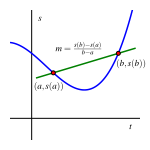
\includegraphics[width=0.5\linewidth]{images/1_1_Summary}
\caption{The graph of position function \(s\) together with the line through \((a,s(a))\) and \((b,s(b))\) whose slope is \(m = \frac{s(b)-s(a)}{b-a}\).  The line's slope is the average rate of change of \(s\) on the interval \([a,b]\).\label{F-1-1-Summary}}
\end{figure}
%
\item{}Given a moving object whose position at time \(t\) is given by a function \(s\), the average velocity of the object on the time interval \([a,b]\) is given by \(AV_{[a,b]} = \frac{s(b) - s(a)}{b-a}\). Viewing the interval \([a,b]\) as having the form \([a,a+h]\), we equivalently compute average velocity by the formula \(AV_{[a,a+h]} = \frac{s(a+h) - s(a)}{h}\).%
\item{}The instantaneous velocity of a moving object at a fixed time is estimated by considering average velocities on shorter and shorter time intervals that contain the instant of interest.%
\end{itemize}
\typeout{************************************************}
\typeout{Exercises 1.1.5 Exercises}
\typeout{************************************************}
\subsection[{Exercises}]{Exercises}\label{ez-1-1}
\begin{exerciselist}
\item[1.]\hypertarget{ez-1-1-WW1}{}\mbox{}\\ % hack to move box after heading
\begin{mdframed}
{}\par\vspace*{2ex}%
{\tiny\ttfamily\noindent
Library/Michigan/Chap2Sec1/Q17.pg\\Seed: \hfill}\end{mdframed}
\item[2.]\hypertarget{ez-1-1-WW2}{}\mbox{}\\ % hack to move box after heading
\begin{mdframed}
{}\par\vspace*{2ex}%
{\tiny\ttfamily\noindent
Library/LoyolaChicago/Precalc/Chap1Sec2/Q14.pg\\Seed: \hfill}\end{mdframed}
\item[3.]\hypertarget{ez-1-1-WW3}{}\mbox{}\\ % hack to move box after heading
\begin{mdframed}
{}\par\vspace*{2ex}%
{\tiny\ttfamily\noindent
Library/LoyolaChicago/Precalc/Chap1Sec2/Q16.pg\\Seed: \hfill}\end{mdframed}
\item[4.]\hypertarget{ez-1-1-WW4}{}\mbox{}\\ % hack to move box after heading
\begin{mdframed}
{}\par\vspace*{2ex}%
{\tiny\ttfamily\noindent
Library/LoyolaChicago/Precalc/Chap1Sec2/Q07.pg\\Seed: \hfill}\end{mdframed}
\item[5.]\hypertarget{ez-1-1-WW5}{}\mbox{}\\ % hack to move box after heading
\begin{mdframed}
{}\par\vspace*{2ex}%
{\tiny\ttfamily\noindent
Library/Michigan/Chap2Sec1/Q13.pg\\Seed: \hfill}\end{mdframed}
\item[6.]\hypertarget{ez-1-1-Bungee}{}A bungee jumper dives from a tower at time \(t=0\). Her height \(h\) (measured in feet) at time \(t\) (in seconds) is given by the graph in \hyperref[F-1-1-Ez1]{Figure~\ref{F-1-1-Ez1}}.
          %
\leavevmode%
\begin{figure}
\centering
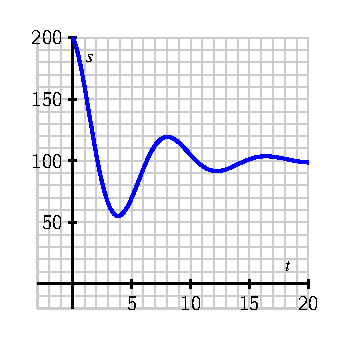
\includegraphics[width=0.5\linewidth]{images/1_1_Ez1}
\caption{A bungee jumper's height function.\label{F-1-1-Ez1}}
\end{figure}
\par

            In this problem, you may base your answers on estimates from the graph or use the fact that the jumper's height function is given by \(s(t) = 100\cos(0.75t) \cdot e^{-0.2t}+100\).
          %
\leavevmode%
\begin{enumerate}[label=\alph*]
\item\hypertarget{li-24}{}What is the change in vertical position of the bungee jumper between \(t=0\) and \(t=15\)?%
\item\hypertarget{li-25}{}Estimate the jumper's average velocity on each of the following time intervals:  \([0,15]\), \([0,2]\), \([1,6]\), and \([8,10]\).  Include units on your answers.%
\item\hypertarget{li-26}{}On what time interval(s) do you think the bungee jumper achieves her greatest average velocity?  Why?%
\item\hypertarget{li-27}{}Estimate the jumper's instantaneous velocity at \(t=5\).  Show your work and explain your reasoning, and include units on your answer.%
\item\hypertarget{li-28}{}Among the average and instantaneous velocities you computed in earlier questions, which are positive and which are negative?  What does negative velocity indicate?%
\end{enumerate}
\par\smallskip
\par\smallskip
\noindent\textbf{Answer.}\hypertarget{answer-4}{}\quad
Exercise Answer%
\par\smallskip
\noindent\textbf{Solution.}\hypertarget{solution-5}{}\quad
Exercise Solution%
\item[7.]\hypertarget{ez-1-1-Diver}{}
            A diver leaps from a 3 meter springboard. His feet leave the board at time \(t=0\), he reaches his maximum height of 4.5 m at \(t = 1.1\) seconds, and enters the water at \(t = 2.45\). Once in the water, the diver coasts to the bottom of the pool (depth 3.5 m), touches bottom at \(t=7\), rests for one second, and then pushes off the bottom. From there he coasts to the surface, and takes his first breath at \(t=13\).
          %
\leavevmode%
\begin{enumerate}[label=\alph*]
\item\hypertarget{li-29}{}Let \(s(t)\) denote the function that gives the height of the diver's feet (in meters) above the water at time \(t\).  (Note that the ``height'' of the bottom of the pool is \(-3.5\) meters.)  Sketch a carefully labeled graph of \(s(t)\) on the provided axes in \hyperref[F-1-1-Ez2]{Figure~\ref{F-1-1-Ez2}}.  Include scale and units on the vertical axis.  Be as detailed as possible.%
% group protects changes to lengths, releases boxes (?)
{% begin: group for a single side-by-side
% set panel max height to practical minimum, created in preamble
\setlength{\panelmax}{0pt}
\newsavebox{\panelboxDimage}
\savebox{\panelboxDimage}{
\includegraphics[width=0.5\linewidth]{images/1_1_Ez2a}
}
\newlength{\phDimage}\setlength{\phDimage}{\ht\panelboxDimage+\dp\panelboxDimage}
\settototalheight{\phDimage}{\usebox{\panelboxDimage}}
\setlength{\panelmax}{\maxof{\panelmax}{\phDimage}}
\newsavebox{\panelboxEimage}
\savebox{\panelboxEimage}{
\includegraphics[width=0.5\linewidth]{images/1_1_Ez2b}
}
\newlength{\phEimage}\setlength{\phEimage}{\ht\panelboxEimage+\dp\panelboxEimage}
\settototalheight{\phEimage}{\usebox{\panelboxEimage}}
\setlength{\panelmax}{\maxof{\panelmax}{\phEimage}}
\leavevmode%
% begin: side-by-side as figure/tabular
% \tabcolsep change local to group
\setlength{\tabcolsep}{0\textwidth}
% @{} suppress \tabcolsep at extremes, so margins behave as intended
\begin{figure}
\begin{tabular}{@{}*{2}{c}@{}}
\begin{minipage}[c][\panelmax][t]{0.5\textwidth}\usebox{\panelboxDimage}\end{minipage}&
\begin{minipage}[c][\panelmax][t]{0.5\textwidth}\usebox{\panelboxEimage}\end{minipage}\end{tabular}
\caption{Axes for plotting \(s(t)\) in part (a) and \(v(t)\) in part (c) of the diver problem.\label{F-1-1-Ez2}}
\end{figure}
% end: side-by-side as tabular/figure
}% end: group for a single side-by-side
\item\hypertarget{li-30}{}Based on your graph in (a), what is the average velocity of the diver between \(t = 2.45\) and \(t=7\)?  Is his average velocity the same on every time interval within \([2.45,7]\)?%
\item\hypertarget{li-31}{}Let the function \(v(t)\) represent the \emph{instantaneous vertical velocity} of the diver at time \(t\) (i.e.~the speed at which the height function \(s(t)\) is changing; note that velocity in the upward direction is positive, while the velocity of a falling object is negative).  Based on your understanding of the diver's behavior, as well as your graph of the position function, sketch a carefully labeled graph of \(v(t)\) on the axes provided  in \hyperref[F-1-1-Ez2]{Figure~\ref{F-1-1-Ez2}}.  Include scale and units on the vertical axis.  Write several sentences that explain how you constructed your graph, discussing when you expect \(v(t)\) to be zero, positive, negative, relatively large, and relatively small.%
\item\hypertarget{li-32}{}Is there a connection between the two graphs that you can describe?  What can you say about the velocity graph when the height function is increasing?  decreasing?  Make as many observations as you can.%
\end{enumerate}
\par\smallskip
\par\smallskip
\noindent\textbf{Answer.}\hypertarget{answer-5}{}\quad
Exercise Answer%
\par\smallskip
\noindent\textbf{Solution.}\hypertarget{solution-6}{}\quad
Exercise Solution%
\item[8.]\hypertarget{exercise-8}{} According to the U.S. census, the population of the city of Grand Rapids, MI, was 181,843 in 1980; 189,126 in 1990; and 197,800 in 2000.
          %
\leavevmode%
\begin{enumerate}[label=\alph*]
\item\hypertarget{li-33}{}Between 1980 and 2000, by how many people did the population of Grand Rapids grow?%
\item\hypertarget{li-34}{}In an average year between 1980 and 2000, by how many people did the population of Grand Rapids grow?%
\item\hypertarget{li-35}{}Just like we can find the average velocity of a moving body by computing change in position over change in time, we can compute the average rate of change of any function \(f\).  In particular, the \emph{average rate of change} of a function \(f\) over an interval \([a,b]\) is the quotient
              \begin{equation*}
              \frac{f(b)-f(a)}{b-a}.
              \end{equation*}
              What does the quantity \(\frac{f(b)-f(a)}{b-a}\) measure on the graph of \(y = f(x)\) over the interval \([a,b]\)?%
\item\hypertarget{li-36}{}Let \(P(t)\) represent the population of Grand Rapids at time \(t\), where \(t\) is measured in years from January 1, 1980.  What is the average rate of change of \(P\) on the interval \(t = 0\) to \(t = 20\)?  What are the units on this quantity?%
\item\hypertarget{li-37}{}If we assume the population of Grand Rapids is growing at a rate of approximately 4\% per decade,  we can model the population function with the formula 
              \begin{equation*}
              P(t) = 181843 (1.04)^{t/10}.
              \end{equation*}
                 Use this formula to compute the average rate of change of the population on the intervals \([5,10]\), \([5,9]\), \([5,8]\), \([5,7]\), and \([5,6]\).%
\item\hypertarget{li-38}{}How fast do you think the population of Grand Rapids was changing on January 1, 1985?  Said differently, at what rate do you think people were being added to the population of Grand Rapids as of January 1, 1985?  How many additional people should the city have expected in the following year?  Why?%
\end{enumerate}
\par\smallskip
\par\smallskip
\noindent\textbf{Answer.}\hypertarget{answer-6}{}\quad
Exercise Answer%
\par\smallskip
\noindent\textbf{Solution.}\hypertarget{solution-7}{}\quad
Exercise Solution%
\end{exerciselist}
\typeout{************************************************}
\typeout{Section 1.2 The notion of limit}
\typeout{************************************************}
\section[{The notion of limit}]{The notion of limit}\label{sec-1-2-lim}
\typeout{************************************************}
\typeout{Introduction  }
\typeout{************************************************}

\emph{Motivating Questions}
%
\leavevmode%
\begin{itemize}[label=\textbullet]
\item{}What is the mathematical notion of \emph{limit} and what role do limits play in the study of functions?%
\item{}What is the meaning of the notation \(\lim_{x \to a} f(x) = L\)?%
\item{}How do we go about determining the value of the limit of a function at a point?%
\item{}How does the notion of limit allow us to move from average velocity to instantaneous velocity?%
\end{itemize}
\par

Functions are at the heart of mathematics: a function is a process or rule that associates each individual input to exactly one corresponding output. Students learn in courses prior to calculus that there are many different ways to represent functions, including through formulas, graphs, tables, and even words. For example, the squaring function can be thought of in any of these ways. In words, the squaring function takes any real number \(x\) and computes its square. The formulaic and graphical representations go hand in hand, as \(y = f(x) = x^2\) is one of the simplest curves to graph. Finally, we can also partially represent this function through a table of values, essentially by listing some of the ordered pairs that lie on the curve, such as \((-2,4)\), \((-1,1)\), \((0,0)\), \((1,1)\), and \((2,4)\).
%
\par

Functions are especially important in calculus because they often model important phenomena -- the location of a moving object at a given time, the rate at which an automobile is consuming gasoline at a certain velocity, the reaction of a patient to the size of a dose of a drug -- and calculus can be used to study how these output quantities change in response to changes in the input variable. Moreover, thinking about concepts like average and instantaneous velocity leads us naturally from an initial function to a related, sometimes more complicated function. As one example of this, think about the falling ball whose position function is given by \(s(t) = 64 - 16t^2\) and the average velocity of the ball on the interval \([1,x]\). Observe that
%
\begin{equation*}
AV_{[1,x]} = \frac{s(x) - s(1)}{x-1} = \frac{(64-16x^2) - (64-16)}{x-1} = \frac{16 - 16x^2}{x-1}.
\end{equation*}\par

Now, two things are essential to note: this average velocity depends on \(x\) (indeed, \(AV_{[1,x]}\) is a function of \(x\)), and our most focused interest in this function occurs near \(x = 1\), which is where the function is not defined. Said differently, the function \(g(x) = \frac{16 - 16x^2}{x-1}\) tells us the average velocity of the ball on the interval from \(t = 1\) to \(t = x\), and if we are interested in the instantaneous velocity of the ball when \(t = 1\), we'd like to know what happens to \(g(x)\) as \(x\) gets closer and closer to \(1\). At the same time, \(g(1)\) is not defined, because it leads to the quotient \(0/0\).
%
\par

This is where the idea of \emph{limits} comes in. By using a limit, we'll be able to allow \(x\) to get arbitrarily close, but not equal, to \(1\) and fully understand the behavior of \(g(x)\) near this value. We'll develop key language, notation, and conceptual understanding in what follows, but for now we consider a preliminary activity that uses the graphical interpretation of a function to explore points on a graph where interesting behavior occurs.
%
\typeout{************************************************}
\typeout{Subsection 1.2.1 Preview Activity}
\typeout{************************************************}
\subsection[{Preview Activity}]{Preview Activity}\label{PA-1-2}

    Suppose that \(g\) is the function given by the graph shown in \hyperref[F-1-2-PA1]{Figure~\ref{F-1-2-PA1}}. Use the graph to answer each of the following questions.
    %
\leavevmode%
\begin{enumerate}[label=\alph*]
\item\hypertarget{li-43}{}Determine the values \(g(-2)\), \(g(-1)\), \(g(0)\), \(g(1)\), and \(g(2)\), if defined.  If the function value is not defined, explain what feature of the graph tells you this.%
\item\hypertarget{li-44}{}For each of the values \(a = -1\), \(a = 0\), and \(a = 2\), complete the following sentence: ``As \(x\) gets closer and closer (but not equal) to \(a\), \(g(x)\) gets as close as we want to ... .''%
\item\hypertarget{li-45}{}What happens as \(x\) gets closer and closer (but not equal) to \(a = 1\)?  Does the function \(g(x)\) get as close as we would like to a single value?%
\end{enumerate}
\leavevmode%
\begin{figure}
\centering
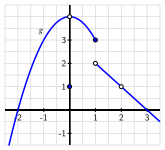
\includegraphics[width=0.5\linewidth]{images/1_2_PA1}
\caption{Graph of \(y = g(x)\) for \hyperref[PA-1-2]{Preview Activity~\ref{PA-1-2}}.\label{F-1-2-PA1}}
\end{figure}
\typeout{************************************************}
\typeout{Subsection 1.2.2 The Notion of Limit}
\typeout{************************************************}
\subsection[{The Notion of Limit}]{The Notion of Limit}\label{subsection-6}

Limits can be thought of as a way to study the tendency or trend of a function as the input variable approaches a fixed value, or even as the input variable increases or decreases without bound. We put off the study of the latter idea until further along in the course when we will have some helpful calculus tools for understanding the end behavior of functions. Here, we focus on what it means to say that ``a function \(f\) has limit \(L\) as \(x\) approaches \(a\).'' To begin, we think about a recent example.
%
\par

In \hyperref[PA-1-2]{Preview Activity~\ref{PA-1-2}}, we saw that for the given function \(g\), as \(x\) gets closer and closer (but not equal) to 0, \(g(x)\) gets as close as we want to the value 4. At first, this may feel counterintuitive, because the value of \(g(0)\) is \(1\), not \(4\). By their very definition, limits regard the behavior of a function \emph{arbitrarily close to} a fixed input, but the value of the function \emph{at} the fixed input does not matter. More formally\footnote{What follows here is not what mathematicians consider the formal definition of a limit.  To be completely precise, it is necessary to quantify both what it means to say ``as close to \(L\) as we like'' and ``sufficiently close to \(a\).''  That can be accomplished through what is traditionally called the epsilon-delta definition of limits.  The definition presented here is sufficient for the purposes of this text.\label{fn-1}}, we say the following.
%
\begin{definition}[{}]\label{definition-1}

    Given a function \(f\), a fixed input \(x = a\), and a real number \(L\), we say that \(f\) has limit \index{} \(L\) as \(x\) approaches \(a\), and write
    %
\begin{equation*}
    \lim_{x \to a} f(x) = L
    \end{equation*}\par

    provided that we can make \(f(x)\) as close to \(L\) as we like by taking \(x\) sufficiently close (but not equal) to \(a\). If we cannot make \(f(x)\) as close to a single value as we would like as \(x\) approaches \(a\), then we say that \(f\) does not have a limit as \(x\) approaches \(a\).
    %
\end{definition}
\par

For the function \(g\) pictured in \hyperref[F-1-2-PA1]{Figure~\ref{F-1-2-PA1}}, we can make the following observations:
%
\begin{equation*}
 \lim_{x \to -1} g(x) = 3, \  \lim_{x \to 0} g(x) = 4, \ \mbox{and}  \  \lim_{x \to 2} g(x) = 1,
\end{equation*}\par

but \(g\) does not have a limit as \(x \to 1\). When working graphically, it suffices to ask if the function approaches a single value from each side of the fixed input, while understanding that the function value right at the fixed input is irrelevant. This reasoning explains the values of the first three stated limits. In a situation such as the jump in the graph of \(g\) at \(x = 1\), the issue is that if we approach \(x = 1\) from the left, the function values tend to get as close to 3 as we'd like, but if we approach \(x = 1\) from the right, the function values get as close to 2 as we'd like, and there is no single number that all of these function values approach. This is why the limit of \(g\) does not exist at \(x = 1\).
%
\par

For any function \(f\), there are typically three ways to answer the question ``does \(f\) have a limit at \(x = a\), and if so, what is the limit?'' The first is to reason graphically as we have just done with the example from \hyperref[PA-1-2]{Preview Activity~\ref{PA-1-2}}. If we have a formula for \(f(x)\), there are two additional possibilities: (1) evaluate the function at a sequence of inputs that approach \(a\) on either side, typically using some sort of computing technology, and ask if the sequence of outputs seems to approach a single value; (2) use the algebraic form of the function to understand the trend in its output as the input values approach \(a\). The first approach only produces an approximation of the value of the limit, while the latter can often be used to determine the limit exactly. The following example demonstrates both of these approaches, while also using the graphs of the respective functions to help confirm our conclusions.
%
\begin{example}[Limits of Two Functions
  ]\label{Ex-1-2-Limits}

    For each of the following functions, we'd like to know whether or not the function has a limit at the stated \(a\)-values. Use both numerical and algebraic approaches to investigate and, if possible, estimate or determine the value of the limit. Compare the results with a careful graph of the function on an interval containing the points of interest.
    %
\leavevmode%
\begin{enumerate}[label=\alph*]
\item\hypertarget{li-46}{}\(f(x) = \frac{4-x^2}{x+2}\); \(a = -1\), \(a = -2\)%
\item\hypertarget{li-47}{}\(g(x) = \sin\left(\frac{\pi}{x}\right)\); \(a = 3\), \(a = 0\)%
\end{enumerate}
\par\medskip\noindent%
\textbf{Solution.}\quad 
  We first construct a graph of \(f\) along with tables of values near \(a = -1\) and \(a = -2\).
  %
% group protects changes to lengths, releases boxes (?)
{% begin: group for a single side-by-side
% set panel max height to practical minimum, created in preamble
\setlength{\panelmax}{0pt}
\newsavebox{\panelboxAtabular}
\savebox{\panelboxAtabular}{
\raisebox{\depth}{\parbox{0.333333333333333\textwidth}{\centering\begin{tabular}{ArAlAl}\hrulethin
\(x\)&\(f(x)\)\tabularnewline\hrulethin
\(-0.9\)&\(2.9\)\tabularnewline\hrulethin
\(-0.99\)&\(2.99\)\tabularnewline\hrulethin
\(-0.999\)&\(2.999\)\tabularnewline\hrulethin
\(-0.9999\)&\(2.9999\)\tabularnewline\hrulethin
\(-1.1\)&\(3.1\)\tabularnewline\hrulethin
\(-1.01\)&\(3.01\)\tabularnewline\hrulethin
\(-1.001\)&\(3.001\)\tabularnewline\hrulethin
\(-1.0001\)&\(3.0001\)\tabularnewline\hrulethin
\end{tabular}
}}}
\newlength{\phAtabular}\setlength{\phAtabular}{\ht\panelboxAtabular+\dp\panelboxAtabular}
\settototalheight{\phAtabular}{\usebox{\panelboxAtabular}}
\setlength{\panelmax}{\maxof{\panelmax}{\phAtabular}}
\newsavebox{\panelboxBtabular}
\savebox{\panelboxBtabular}{
\raisebox{\depth}{\parbox{0.333333333333333\textwidth}{\centering\begin{tabular}{ArAlAl}\hrulethin
\(x\)&\(f(x)\)\tabularnewline\hrulethin
\(-1.9\)&\(3.9\)\tabularnewline\hrulethin
\(-1.99\)&\(3.99\)\tabularnewline\hrulethin
\(-1.999\)&\(3.999\)\tabularnewline\hrulethin
\(-1.9999\)&\(3.9999\)\tabularnewline\hrulethin
\(-2.1\)&\(4.1\)\tabularnewline\hrulethin
\(-2.01\)&\(4.01\)\tabularnewline\hrulethin
\(-2.001\)&\(4.001\)\tabularnewline\hrulethin
\(-2.0001\)&\(4.0001\)\tabularnewline\hrulethin
\end{tabular}
}}}
\newlength{\phBtabular}\setlength{\phBtabular}{\ht\panelboxBtabular+\dp\panelboxBtabular}
\settototalheight{\phBtabular}{\usebox{\panelboxBtabular}}
\setlength{\panelmax}{\maxof{\panelmax}{\phBtabular}}
\newsavebox{\panelboxGimage}
\savebox{\panelboxGimage}{
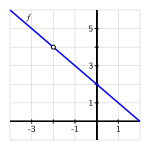
\includegraphics[width=0.333333333333333\linewidth]{images/1_2_Ex1f}
}
\newlength{\phGimage}\setlength{\phGimage}{\ht\panelboxGimage+\dp\panelboxGimage}
\settototalheight{\phGimage}{\usebox{\panelboxGimage}}
\setlength{\panelmax}{\maxof{\panelmax}{\phGimage}}
\leavevmode%
% begin: side-by-side as figure/tabular
% \tabcolsep change local to group
\setlength{\tabcolsep}{0\textwidth}
% @{} suppress \tabcolsep at extremes, so margins behave as intended
\begin{figure}
\begin{tabular}{@{}*{3}{c}@{}}
\begin{minipage}[c][\panelmax][t]{0.333333333333333\textwidth}\usebox{\panelboxAtabular}\end{minipage}&
\begin{minipage}[c][\panelmax][t]{0.333333333333333\textwidth}\usebox{\panelboxBtabular}\end{minipage}&
\begin{minipage}[c][\panelmax][t]{0.333333333333333\textwidth}\usebox{\panelboxGimage}\end{minipage}\tabularnewline
\parbox[t]{0.333333333333333\textwidth}{\subcaption{Table of \(f\) values near \(x=-1\).\label{table-1-F-1-2-Ex1f}}
}&
\parbox[t]{0.333333333333333\textwidth}{\subcaption{Table of \(f\) values near \(x=-2\).\label{table-2-F-1-2-Ex1f}}
}&
\parbox[t]{0.333333333333333\textwidth}{\subcaption{Plot of \(f(x)\) on the interval \([-4,2]\)\label{plot-F-1-2-Ex1f}}
}\end{tabular}
\caption{Tables and graph for \(f(x) = \frac{4-x^2}{x+2}\). \label{F-1-2-Ex1f}}
\end{figure}
% end: side-by-side as tabular/figure
}% end: group for a single side-by-side
\par

    From \hyperref[table-1-F-1-2-Ex1f]{Table~\ref{table-1-F-1-2-Ex1f}}, it appears that we can make \(f\) as close as we want to 3 by taking \(x\) sufficiently close to \(-1\), which suggests that \(\lim_{x \to -1} f(x) = 3\). This is also consistent with the graph of \(f\). To see this a bit more rigorously and from an algebraic point of view, consider the formula for \(f\): \(f(x) = \frac{4-x^2}{x+2}\). The numerator and denominator are each polynomial functions, which are among the most well-behaved functions that exist. Formally, such functions are \emph{continuous}\footnote{See {$\langle\langle$Unresolved xref, reference "sec-1-7-lim-cont-diff"; check spelling or use "provisional" attribute$\rangle\rangle$} for more on the notion of continuity.\label{fn-2}}, which means that the limit of the function at any point is equal to its function value. Here, it follows that as \(x \to -1\), \((4-x^2) \to (4 - (-1)^2) = 3\), and \((x+2) \to (-1 + 2) = 1\), so as \(x \to -1\), the numerator of \(f\) tends to 3 and the denominator tends to 1, hence \(\lim_{x \to -1} f(x) = \frac{3}{1} = 3\).
    %
\par

    The situation is more complicated when \(x \to -2\), due in part to the fact that \(f(-2)\) is not defined. If we attempt to use a similar algebraic argument regarding the numerator and denominator, we observe that as \(x \to -2\), \((4-x^2) \to (4 - (-2)^2) = 0\), and \((x+2) \to (-2 + 2) = 0\), so as \(x \to -2\), the numerator of \(f\) tends to 0 and the denominator tends to 0. We call \(0/0\) an \emph{indeterminate form}\index{} and will revisit several important issues surrounding such quantities later in the course. For now, we simply observe that this tells us there is somehow more work to do. From \hyperref[table-2-F-1-2-Ex1f]{Table~\ref{table-2-F-1-2-Ex1f}} and \hyperref[plot-F-1-2-Ex1f]{Figure~\ref{plot-F-1-2-Ex1f}}, it appears that \(f\) should have a limit of \(4\) at \(x = -2\). To see algebraically why this is the case, let's work directly with the form of \(f(x)\). Observe that
    %
\begin{align*}
\lim_{x \to -2} f(x) = \amp  \lim_{x \to -2} \frac{4-x^2}{x+2}\\
                     = \amp  \lim_{x \to -2} \frac{(2-x)(2+x)}{x+2}.
\end{align*}\par

    At this point, it is important to observe that since we are taking the limit as \(x \to -2\), we are considering \(x\) values that are close, but not equal, to \(-2\). Since we never actually allow \(x\) to equal \(-2\), the quotient \(\frac{2+x}{x+2}\) has value 1 for every possible value of \(x\). Thus, we can simplify the most recent expression above, and now find that
    %
\begin{equation*}
    \lim_{x \to -2} f(x) = \lim_{x \to -2} 2-x.
    \end{equation*}\par

    Because \(2-x\) is simply a linear function, this limit is now easy to determine, and its value clearly is \(4\). Thus, from several points of view we've seen that \(lim_{x \to -2} f(x) = 4.\)
    %
\par

    Next we turn to the function \(g\), and construct two tables and a graph.
    %
% group protects changes to lengths, releases boxes (?)
{% begin: group for a single side-by-side
% set panel max height to practical minimum, created in preamble
\setlength{\panelmax}{0pt}
\newsavebox{\panelboxCtabular}
\savebox{\panelboxCtabular}{
\raisebox{\depth}{\parbox{0.333333333333333\textwidth}{\centering\begin{tabular}{ArAlAl}\hrulethin
\(x\)&\(g(x)\)\tabularnewline\hrulethin
\(2.9\)&\(0.84864\)\tabularnewline\hrulethin
\(2.99\)&\(0.86428\)\tabularnewline\hrulethin
\(2.999\)&\(0.86585\)\tabularnewline\hrulethin
\(2.9999\)&\(0.86601\)\tabularnewline\hrulethin
\(-3.1\)&\(0.88351\)\tabularnewline\hrulethin
\(3.01\)&\(0.86777\)\tabularnewline\hrulethin
\(3.001\)&\(0.86620\)\tabularnewline\hrulethin
\(3.0001\)&\(0.86604\)\tabularnewline\hrulethin
\end{tabular}
}}}
\newlength{\phCtabular}\setlength{\phCtabular}{\ht\panelboxCtabular+\dp\panelboxCtabular}
\settototalheight{\phCtabular}{\usebox{\panelboxCtabular}}
\setlength{\panelmax}{\maxof{\panelmax}{\phCtabular}}
\newsavebox{\panelboxDtabular}
\savebox{\panelboxDtabular}{
\raisebox{\depth}{\parbox{0.333333333333333\textwidth}{\centering\begin{tabular}{ArAlAl}\hrulethin
\(x\)&\(g(x)\)\tabularnewline\hrulethin
\(-0.1\)&\(0\)\tabularnewline\hrulethin
\(-0.01\)&\(0\)\tabularnewline\hrulethin
\(-0.001\)&\(0\)\tabularnewline\hrulethin
\(-0.0001\)&\(0\)\tabularnewline\hrulethin
\(0.1\)&\(0\)\tabularnewline\hrulethin
\(0.01\)&\(0\)\tabularnewline\hrulethin
\(0.001\)&\(0\)\tabularnewline\hrulethin
\(0.0001\)&\(0\)\tabularnewline\hrulethin
\end{tabular}
}}}
\newlength{\phDtabular}\setlength{\phDtabular}{\ht\panelboxDtabular+\dp\panelboxDtabular}
\settototalheight{\phDtabular}{\usebox{\panelboxDtabular}}
\setlength{\panelmax}{\maxof{\panelmax}{\phDtabular}}
\newsavebox{\panelboxHimage}
\savebox{\panelboxHimage}{
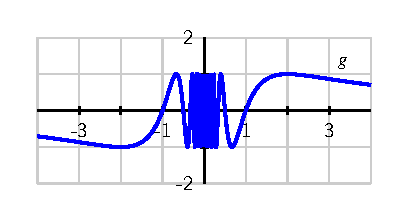
\includegraphics[width=0.333333333333333\linewidth]{images/1_2_Ex1g}
}
\newlength{\phHimage}\setlength{\phHimage}{\ht\panelboxHimage+\dp\panelboxHimage}
\settototalheight{\phHimage}{\usebox{\panelboxHimage}}
\setlength{\panelmax}{\maxof{\panelmax}{\phHimage}}
\leavevmode%
% begin: side-by-side as figure/tabular
% \tabcolsep change local to group
\setlength{\tabcolsep}{0\textwidth}
% @{} suppress \tabcolsep at extremes, so margins behave as intended
\begin{figure}
\begin{tabular}{@{}*{3}{c}@{}}
\begin{minipage}[c][\panelmax][t]{0.333333333333333\textwidth}\usebox{\panelboxCtabular}\end{minipage}&
\begin{minipage}[c][\panelmax][t]{0.333333333333333\textwidth}\usebox{\panelboxDtabular}\end{minipage}&
\begin{minipage}[c][\panelmax][t]{0.333333333333333\textwidth}\usebox{\panelboxHimage}\end{minipage}\tabularnewline
\parbox[t]{0.333333333333333\textwidth}{\subcaption{Table of \(g\) values near \(x=3\).\label{table-1-F-1-2-Ex1g}}
}&
\parbox[t]{0.333333333333333\textwidth}{\subcaption{Table of certain \(g\) values near \(x=0\).\label{table-2-F-1-2-Ex1g}}
}&
\parbox[t]{0.333333333333333\textwidth}{\subcaption{Plot of \(g(x)\) on the interval \([-4,4]\)\label{plot-F-1-2-Ex1g}}
}\end{tabular}
\caption{Tables and graph for \(g(x) = \sin(\frac{\pi}{x})\). \label{F-1-2-Ex1g}}
\end{figure}
% end: side-by-side as tabular/figure
}% end: group for a single side-by-side
\par

    First, as \(x \to 3\), it appears from the data (and the graph) that the function is approaching approximately \(0.866025\). To be precise, we have to use the fact that \(\frac{\pi}{x} \to \frac{\pi}{3}\), and thus we find that \(g(x) = \sin(\frac{\pi}{x}) \to \sin(\frac{\pi}{3})\) as \(x \to 3\). The exact value of \(\sin(\frac{\pi}{3})\) is \(\frac{\sqrt{3}}{2}\), which is approximately 0.8660254038. Thus, we see that
    %
\begin{equation*}
    \lim_{x \to 3} g(x) = \frac{\sqrt{3}}{2}.
    \end{equation*}\par

    As \(x \to 0\), we observe that \(\frac{\pi}{x}\) does not behave in an elementary way. When \(x\) is positive and approaching zero, we are dividing by smaller and smaller positive values, and \(\frac{\pi}{x}\) increases without bound. When \(x\) is negative and approaching zero, \(\frac{\pi}{x}\) decreases without bound. In this sense, as we get close to \(x = 0\), the inputs to the sine function are growing rapidly, and this leads to wild oscillations in the graph of \(g\). It is an instructive exercise to plot the function \(g(x) = \sin\left(\frac{\pi}{x}\right)\) with a graphing utility and then zoom in on \(x = 0\). Doing so shows that the function never settles down to a single value near the origin and suggests that \(g\) does not have a limit at \(x = 0\).
    %
\par

    How do we reconcile this with the righthand table above, which seems to suggest that the limit of \(g\) as \(x\) approaches \(0\) may in fact be \(0\)? Here we need to recognize that the data misleads us because of the special nature of the sequence \(\{0.1, 0.01, 0.001, \ldots\}\): when we evaluate \(g(10^{-k})\), we get \(g(10^{-k}) = \sin\left(\frac{\pi}{10^{-k}}\right) = \sin(10^k \pi) = 0\) for each positive integer value of \(k\). But if we take a different sequence of values approaching zero, say \(\{0.3, 0.03, 0.003, \ldots\}\), then we find that
    %
\begin{equation*}
    g(3 \cdot 10^{-k}) = \sin\left(\frac{\pi}{3 \cdot 10^{-k}}\right) = \sin\left(\frac{10^k \pi}{3}\right) = \frac{\sqrt{3}}{2} \approx 0.866025.
    \end{equation*}\par

    That sequence of data would suggest that the value of the limit is \(\frac{\sqrt{3}}{2}\). Clearly the function cannot have two different values for the limit, and this shows that \(g\) has no limit as \(x \to 0\).
    %
\end{example}
\par

    An important lesson to take from \hyperref[Ex-1-2-Limits]{Example~\ref{Ex-1-2-Limits}} is that tables can be misleading when determining the value of a limit. While a table of values is useful for investigating the possible value of a limit, we should also use other tools to confirm the value, if we think the table suggests the limit exists.
    %
\begin{activity}[Evaluating Three Limits]\label{act-1-2-1}

          Estimate the value of each of the following limits by constructing appropriate tables of values. Then determine the exact value of the limit by using algebra to simplify the function. Finally, plot each function on an appropriate interval to check your result visually.
          %
\leavevmode%
\begin{enumerate}[label=\alph*]
\item\hypertarget{li-48}{}\(\lim_{x \to 1} \frac{x^2 - 1}{x-1}\)%
\item\hypertarget{li-49}{}\(\lim_{x \to 0} \frac{(2+x)^3 - 8}{x}\)%
\item\hypertarget{li-50}{}\(\lim_{x \to 0} \frac{\sqrt{x+1} - 1}{x}\)%
\end{enumerate}
\leavevmode%
\begin{enumerate}[label=\alph*]
\item\hypertarget{li-51}{}\((x^2 - 1)\) can be factored.%
\item\hypertarget{li-52}{}Expand the expression \((2+x)^3\), and then combine like terms in the numerator.%
\item\hypertarget{li-53}{}Try multiplying the given function by this fancy form of 1: \(\frac{\sqrt{x+1} + 1}{\sqrt{x+1} + 1}\).%
\end{enumerate}
\leavevmode%
\begin{enumerate}[label=\alph*lpha]
\item\hypertarget{li-54}{}\(2\).%
\item\hypertarget{li-55}{}\(12\).%
\item\hypertarget{li-56}{}\(\frac{1}{2}.\)%
\end{enumerate}
\par\medskip\noindent%
\textbf{Solution.}\quad 
        Estimating the values of the limits with tables is straightforward and should suggest the exact values stated below.
        %
\leavevmode%
\begin{enumerate}[label=\alph*lpha]
\item\hypertarget{li-57}{}\(\lim_{x \to 1} \frac{x^2 - 1}{x-1} = \lim_{x \to 1} \frac{(x+1)(x-1)}{x-1} = \lim_{x \to 1} (x+1) = 2\).%
\item\hypertarget{li-58}{}\(\lim_{x \to 0} \frac{(2+x)^3 - 8}{x} = \lim_{x \to 0} \frac{8 + 12x + 6x^2 + x^3 - 8}{x} = \lim_{x \to 0} \frac{12x + 6x^2 + x^3}{x} =  \lim_{x \to 0} (12 + 6x + x^2) = 12\).%
\item\hypertarget{li-59}{}\(\lim_{x \to 0} \frac{\sqrt{x+1} - 1}{x} = \lim_{x \to 0} \frac{\sqrt{x+1} - 1}{x} \cdot \frac{\sqrt{x+1} + 1}{\sqrt{x+1} + 1} = \lim_{x \to 0} \frac{x+1-1}{x(\sqrt{x+1}+1)} = \lim_{x \to 0} \frac{1}{\sqrt{x+1}+1} = \frac{1}{2}.\)%
\end{enumerate}
\end{activity}
\par

    This concludes a rather lengthy introduction to the notion of limits. It is important to remember that our primary motivation for considering limits of functions comes from our interest in studying the rate of change of a function. To that end, we close this section by revisiting our previous work with average and instantaneous velocity and highlighting the role that limits play.
    %
\typeout{************************************************}
\typeout{Subsection 1.2.3 Instantaneous Velocity}
\typeout{************************************************}
\subsection[{Instantaneous Velocity}]{Instantaneous Velocity}\label{subsection-7}

  Suppose that we have a moving object whose position at time \(t\) is given by a function \(s\). We know that the average velocity of the object on the time interval \([a,b]\) is \(AV_{[a,b]} = \frac{s(b)-s(a)}{b-a}.\) We define the \emph{instantaneous velocity} \index{} at \(a\) to be the limit of average velocity as \(b\) approaches \(a\). Note particularly that as \(b \to a\), the length of the time interval gets shorter and shorter (while always including \(a\)). In \hyperref[sec-1-3-derivative-pt]{Section~\ref{sec-1-3-derivative-pt}}, we will introduce a helpful shorthand notation to represent the instantaneous rate of change. For now, we will write \(IV_{t=a}\) for the instantaneous velocity at \(t = a\), and thus
  %
\begin{equation*}
  IV_{t=a} = \lim_{b \to a} AV_{[a,b]} = \lim_{b \to a} \frac{s(b)-s(a)}{b-a}.
  \end{equation*}\par

  Equivalently, if we think of the changing value \(b\) as being of the form \(b = a + h\), where \(h\) is some small number, then we may instead write
  %
\begin{equation*}
  IV_{t=a} = \lim_{h \to 0} AV_{[a,a+h]} = \lim_{h \to 0} \frac{s(a+h)-s(a)}{h}.
  \end{equation*}\par

  Again, the most important idea here is that to compute instantaneous velocity, we take a limit of average velocities as the time interval shrinks. Two different activities offer the opportunity to investigate these ideas and the role of limits further. 
  %
\begin{activity}[A moving object with position \(s(t)=t^2\)]\label{act-1-2-2}

        Consider a moving object whose position function is given by \(s(t) = t^2\), where \(s\) is measured in meters and \(t\) is measured in minutes.
        %
\leavevmode%
\begin{enumerate}[label=\alph*lpha]
\item\hypertarget{li-60}{}Determine the most simplified expression for the average velocity of the object on the interval \([3, 3+h]\), where \(h \gt 0\).%
\item\hypertarget{li-61}{}Determine the average velocity of the object on the interval \([3,3.2]\).  Include units on your answer.%
\item\hypertarget{li-62}{}Determine the instantaneous velocity of the object when \(t = 3\).  Include units on your answer.%
\end{enumerate}
\leavevmode%
\begin{enumerate}[label=\alph*lpha]
\item\hypertarget{li-63}{}\(s(3+h) = (3+h)^2\).%
\item\hypertarget{li-64}{}Recall that \(AV_{[a,b]} = \frac{s(b)-s(a)}{b-a}\).%
\item\hypertarget{li-65}{}Consider \(\lim_{h \to 0} \frac{s(3+h)-s(3)}{h}\) and use your work in (a).%
\end{enumerate}
\leavevmode%
\begin{enumerate}[label=\alph*lpha]
\item\hypertarget{li-66}{}\(6 + h.\)%
\item\hypertarget{li-67}{}\(6.2\) meters/min.%
\item\hypertarget{li-68}{}\(6\) meters per minute.%
\end{enumerate}
\par\medskip\noindent%
\textbf{Solution.}\quad \leavevmode%
\begin{enumerate}[label=\alph*lpha]
\item\hypertarget{li-69}{}Observe that \(AV_{[3, 3+h]} =  \frac{s(3+h)-s(3)}{h} = \frac{(3+h)^2 - 3^2}{h} = \frac{9 + 6h + h^2 - 9}{h} = \frac{6h + h^2}{h} = \frac{h(6 + h)}{h} = 6 + h.\)%
\item\hypertarget{li-70}{}Using the expression just found in (a) with \(h = 0.2\), \(AV_{[3,3.2]} = 6 + 0.2 = 6.2\) meters/min.%
\item\hypertarget{li-71}{}Taking the limit of average velocity and using our work from (a), we find that
  
              \begin{equation*}
              IV_{t = 3} = \lim_{h \to 0} AV_{[3, 3+h]} = \lim_{h \to 0} 6+h = 6,
              \end{equation*}
 
            so the instantaneous velocity of the object when \(t = 3\) is 6 meters per minute.%
\end{enumerate}
\end{activity}
\par

  The closing activity of this section asks you to make some connections among average velocity, instantaneous velocity, and slopes of certain lines.
  %
\begin{activity}[A moving object with position given by a graph]\label{act-1-2-3}

          For the moving object whose position \(s\) at time \(t\) is given by the graph below, answer each of the following questions. Assume that \(s\) is measured in feet and \(t\) is measured in seconds.
          %
\leavevmode%
\begin{figure}
\centering
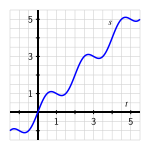
\includegraphics[width=0.5\linewidth]{images/1_2_Act3}
\caption{Plot of the position function \(y = s(t)\) in \hyperref[act-1-2-3]{Activity~\ref{act-1-2-3}}.\label{figure-7}}
\end{figure}
\leavevmode%
\begin{enumerate}[label=\alph*lpha]
\item\hypertarget{li-72}{}Use the graph to estimate the average velocity of the object on each of the following intervals: \([0.5,1]\), \([1.5,2.5]\), \([0,5]\).  Draw each line whose slope represents the average velocity you seek.%
\item\hypertarget{li-73}{}How could you use average velocities or slopes of lines to estimate the instantaneous velocity of the object at a fixed time?%
\item\hypertarget{li-74}{}Use the graph to estimate the instantaneous velocity of the object when \(t = 2\).  Should this instantaneous velocity at \(t = 2\) be greater or less than the average velocity on \([1.5,2.5]\) that you computed in (a)?  Why?%
\end{enumerate}
\leavevmode%
\begin{enumerate}[label=\alph*lpha]
\item\hypertarget{li-75}{}Remember that average velocity on an interval computes the quotient of ``change in \(s\) over change in \(t\).''  This is the slope of the line between the corresponding two points on the graph of \(s\).%
\item\hypertarget{li-76}{}Think about shorter and shorter time intervals and drawing the lines whose slopes represent average velocity.%
\item\hypertarget{li-77}{}Think about zooming in on the graph at \(t = 2\) and drawing a line that, up close, looks just like the curve \(s(t)\).  What is the approximate slope of that line?%
\end{enumerate}
\leavevmode%
\begin{enumerate}[label=\alph*lpha]
\item\hypertarget{li-78}{}The average velocity on \([0.5,1]\) is the slope of the line joining the points \((0.5,s(0.5))\) and \((1,s(1))\), which is \(AV_{[0.5,1]} = \frac{1-1}{1-0.5} = 0\).  On \([1.5,2.5]\), we similarly find \(AV_{[1.5,2.5]} = \frac{3-1}{2.5-1.5} = 2\), and on \([0,5]\), we have \(AV_{[0,5]} = \frac{5-0}{5-0} = 1\).%
\item\hypertarget{li-79}{}Take shorter and shorter time intervals and draw the lines whose slopes represent average velocity.  If those lines' slopes are approaching a single number, that number represents the instantaneous velocity.  For example, to estimate the instantaneous velocity at \(t = 2\), we might consider average velocities on \([2,3]\), \([2,2.5]\), and \([2,2.25]\).%
\item\hypertarget{li-80}{}The instantaneous velocity at \(t = 2\) is greater than the average velocity on \([1.5,2.5]\).%
\end{enumerate}
\par\medskip\noindent%
\textbf{Solution.}\quad \leavevmode%
\begin{enumerate}[label=\alph*lpha]
\item\hypertarget{li-81}{}\(AV_{[0.5,1]} = \frac{1-1}{1-0.5} = 0\), \(AV_{[1.5,2.5]} = \frac{3-1}{2.5-1.5} = 2\), and \(AV_{[0,5]} = \frac{5-0}{5-0} = 1\).%
\item\hypertarget{li-82}{}Take shorter and shorter time intervals and draw the lines whose slopes represent average velocity.  If those lines' slopes are approaching a single number, that number represents the instantaneous velocity.%
\item\hypertarget{li-83}{}If we draw the line through \((2,2)\) and \((2.1,s(2.1))\), it looks like the line's slope is approximately 2.5: if we go over one grid-width, we appear to go up about 2.5.  The slope of this line is clearly greater than the slope of the line through \((1.5, s(1.5))\) and \((2.5, s(2.5))\), which is 2. Hence the instantaneous velocity at \(t = 2\) is greater than the average velocity on \([1.5,2.5]\).%
\end{enumerate}
\end{activity}
\typeout{************************************************}
\typeout{Subsection 1.2.4 Summary}
\typeout{************************************************}
\subsection[{Summary}]{Summary}\label{subsection-8}
\leavevmode%
\begin{itemize}[label=\textbullet]
\item{}Limits enable us to examine trends in function behavior near a specific point. In particular, taking a limit at a given point asks if the function values nearby tend to approach a particular fixed value.%
\item{}When we write \(\lim_{x \to a} f(x) = L\), we read this as saying ``the limit of \(f\) as \(x\) approaches \(a\) is \(L\),'' and this means that we can make the value of \(f(x)\) as close to \(L\) as we want by taking \(x\) sufficiently close (but not equal) to \(a\).%
\item{} If we desire to know \(\lim_{x \to a} f(x)\) for a given value of \(a\) and a known function \(f\), we can estimate this value from the graph of \(f\) or by generating a table of function values that result from a sequence of \(x\)-values that are closer and closer to \(a\). If we want the exact value of the limit, we need to work with the function algebraically and see if we can use familiar properties of known, basic functions to understand how different parts of the formula for \(f\) change as \(x \to a\).%
\item{}The instantaneous velocity of a moving object at a fixed time is found by taking the limit of average velocities of the object over shorter and shorter time intervals that all contain the time of interest.%
\end{itemize}
\typeout{************************************************}
\typeout{Exercises 1.2.5 Exercises}
\typeout{************************************************}
\subsection[{Exercises}]{Exercises}\label{ez-1-2}
\begin{exerciselist}
\item[1.]\hypertarget{ez-1-2-WW1}{}\mbox{}\\ % hack to move box after heading
\begin{mdframed}
{}\par\vspace*{2ex}%
{\tiny\ttfamily\noindent
Library/Michigan/Chap1Sec8/Q01.pg\\Seed: \hfill}\end{mdframed}
\item[2.]\hypertarget{ez-1-2-WW2}{}\mbox{}\\ % hack to move box after heading
\begin{mdframed}
{}\par\vspace*{2ex}%
{\tiny\ttfamily\noindent
Library/ASU-topics/setLimitConcepts/ur_lr_1-5_1.pg\\Seed: \hfill}\end{mdframed}
\item[3.]\hypertarget{ez-1-2-WW3}{}\mbox{}\\ % hack to move box after heading
\begin{mdframed}
{}\par\vspace*{2ex}%
{\tiny\ttfamily\noindent
Library/Michigan/Chap1Sec8/Q03.pg\\Seed: \hfill}\end{mdframed}
\item[4.]\hypertarget{ez-1-2-WW4}{}\mbox{}\\ % hack to move box after heading
\begin{mdframed}
{}\par\vspace*{2ex}%
{\tiny\ttfamily\noindent
Library/Michigan/Chap1Sec8/Q21.pg\\Seed: \hfill}\end{mdframed}
\item[5.]\hypertarget{ez-1-2-WW5}{}\mbox{}\\ % hack to move box after heading
\begin{mdframed}
{}\par\vspace*{2ex}%
{\tiny\ttfamily\noindent
Library/ASU-topics/setLimitConcepts/3-2-34.pg\\Seed: \hfill}\end{mdframed}
\item[6.]\hypertarget{ez-1-2-Rational}{}
          Consider the function whose formula is \(f(x) = \frac{16-x^4}{x^2-4}\).
          %
\leavevmode%
\begin{enumerate}[label=\alph*]
\item\hypertarget{li-88}{}What is the domain of \(f\)?%
\item\hypertarget{li-89}{}Use a sequence of values of \(x\) near \(a = 2\) to estimate the value of \(\lim_{x \to 2} f(x),\)
              if you think the limit exists.  If you think the limit doesn't exist, explain why.%
\item\hypertarget{li-90}{}Use algebra to simplify the expression \(\frac{16-x^4}{x^2-4}\) and hence work to evaluate \(\lim_{x \to 2} f(x)\) exactly, if it exists, or to explain how your work shows the limit fails to exist.  Discuss how your findings compare to your results in (b).%
\item\hypertarget{li-91}{}True or false: \(f(2) = -8\).  Why?%
\item\hypertarget{li-92}{}True or false: \(\frac{16-x^4}{x^2-4} = -4-x^2.\)  Why?  How is this equality connected to your work above with the function \(f\)?%
\item\hypertarget{li-93}{}Based on all of your work above, construct an accurate, labeled graph of \(y = f(x)\) on the interval \([1,3]\), and write a sentence that explains what you now know about \(\lim_{x \to 2} \frac{16-x^4}{x^2-4}\).%
\end{enumerate}
\par\smallskip
\par\smallskip
\noindent\textbf{Answer.}\hypertarget{answer-10}{}\quad
Exercise Answer%
\par\smallskip
\noindent\textbf{Solution.}\hypertarget{solution-12}{}\quad
Exercise Solution%
\item[7.]\hypertarget{ez-1-2-abs-val}{}Let \(g(x) = -\frac{|x+3|}{x+3}\).%
\leavevmode%
\begin{enumerate}[label=\alph*]
\item\hypertarget{li-94}{}What is the domain of \(g\)?%
\item\hypertarget{li-95}{}Use a sequence of values near \(a = -3\) to estimate the value of \(\lim_{x \to -3} g(x),\)
            if you think the limit exists.  If you think the limit doesn't exist, explain why.%
\item\hypertarget{li-96}{}Use algebra to simplify the expression \(\frac{|x+3|}{x+3}\) and hence work to evaluate \(\lim_{x \to -3} g(x)\) exactly, if it exists, or to explain how your work shows the limit fails to exist.  Discuss how your findings compare to your results in (b).  (Hint: \(|a| = a\) whenever \(a \ge 0\), but \(|a| = -a\) whenever \(a \lt  0\).)%
\item\hypertarget{li-97}{}True or false: \(g(-3) = -1\).  Why?%
\item\hypertarget{li-98}{}True or false: \(-\frac{|x+3|}{x+3} = -1.\)  Why?  How is this equality connected to your work above with the function \(g\)?%
\item\hypertarget{li-99}{}Based on all of your work above, construct an accurate, labeled graph of \(y = g(x)\) on the interval \([-4,-2]\), and write a sentence that explains what you now know about \(\lim_{x \to -3} g(x)\).%
\end{enumerate}
\par\smallskip
\par\smallskip
\noindent\textbf{Answer.}\hypertarget{answer-11}{}\quad
Exercise Answer%
\par\smallskip
\noindent\textbf{Solution.}\hypertarget{solution-13}{}\quad
Exercise Solution%
\item[8.]\hypertarget{ez-1-2-Two-Graphs}{}For each of the following prompts, sketch a graph on the provided axes of a function that has the stated properties.
          %
\leavevmode%
\begin{figure}
\centering
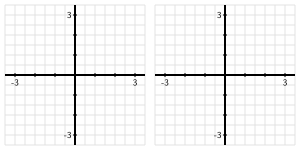
\includegraphics[width=0.5\linewidth]{images/1_2_Ez3}
\caption{Axes for plotting \(y = f(x)\) in (a) and \(y = g(x)\) in (b).\label{F-1-2-Ez3}}
\end{figure}
\leavevmode%
\begin{enumerate}[label=\alph*]
\item\hypertarget{li-100}{}\(y = f(x)\) such that 
                %
\begin{itemize}[label=\textbullet]
\item{}\(f(-2) = 2\) and \(\lim_{x \to -2} f(x) = 1\)%
\item{}\(f(-1) = 3\) and \(\lim_{x \to -1} f(x) = 3\)%
\item{}\(f(1)\) is not defined and \(\lim_{x \to 1} f(x) = 0\)%
\item{}\(f(2) = 1\) and \(\lim_{x \to 2} f(x)\) does not exist.%
\end{itemize}
%
\item\hypertarget{li-105}{}\(y = g(x)\) such that
                %
\begin{itemize}[label=\textbullet]
\item{}\(g(-2) = 3\), \(g(-1) = -1\), \(g(1) = -2\), and \(g(2) = 3\)%
\item{}At \(x = -2, -1, 1\) and \(2\), \(g\) has a limit, and its limit equals the value of the function at that point.%
\item{}\(g(0)\) is not defined and \(\lim_{x \to 0} g(x)\) does not exist.%
\end{itemize}
%
\end{enumerate}
\par\smallskip
\par\smallskip
\noindent\textbf{Answer.}\hypertarget{answer-12}{}\quad
Exercise Answer%
\par\smallskip
\noindent\textbf{Solution.}\hypertarget{solution-14}{}\quad
Exercise Solution%
\item[9.]\hypertarget{ez-1-2-Bungee}{}A bungee jumper dives from a tower at time \(t=0\). Her height \(s\) in feet at time \(t\) in seconds is given by \(s(t) = 100\cos(0.75t) \cdot e^{-0.2t}+100\).
          %
\leavevmode%
\begin{enumerate}[label=\alph*]
\item\hypertarget{li-109}{}Write an expression for the average velocity of the bungee jumper on the interval \([1,1+h]\).%
\item\hypertarget{li-110}{}Use computing technology to estimate the value of the limit as \(h \to 0\) of the quantity you found in (a).
            %
\item\hypertarget{li-111}{}What is the meaning of the value of the limit in (b)?  What are its units?%
\end{enumerate}
\par\smallskip
\par\smallskip
\noindent\textbf{Answer.}\hypertarget{answer-13}{}\quad
Exercise Answer%
\par\smallskip
\noindent\textbf{Solution.}\hypertarget{solution-15}{}\quad
Exercise Solution%
\end{exerciselist}
\typeout{************************************************}
\typeout{Section 1.3 The derivative of a function at a point}
\typeout{************************************************}
\section[{The derivative of a function at a point}]{The derivative of a function at a point}\label{sec-1-3-derivative-pt}
\typeout{************************************************}
\typeout{Introduction  }
\typeout{************************************************}

\emph{Motivating Questions}
%
\leavevmode%
\begin{itemize}[label=\textbullet]
\item{}How is the average rate of change of a function on a given interval defined, and what does this quantity measure?%
\item{}How is the instantaneous rate of change of a function at a particular point defined?  How is the instantaneous rate of change linked to average rate of change?%
\item{}What is the derivative of a function at a given point?  What does this derivative value measure? How do we interpret the derivative value graphically?%
\item{}How are limits used formally in the computation of derivatives?%
\end{itemize}
\par

An idea that sits at the foundations of calculus is the \emph{instantaneous rate of change} of a function. This rate of change is always considered with respect to change in the input variable, often at a particular fixed input value. This is a generalization of the notion of instantaneous velocity and essentially allows us to consider the question ``how do we measure how fast a particular function is changing at a given point?'' When the original function represents the position of a moving object, this instantaneous rate of change is precisely velocity, and might be measured in units such as feet per second. But in other contexts, instantaneous rate of change could measure the number of cells added to a bacteria culture per day, the number of additional gallons of gasoline consumed by going one mile per additional mile per hour in a car's velocity, or the number of dollars added to a mortgage payment for each percentage increase in interest rate. Regardless of the presence of a physical or practical interpretation of a function, the instantaneous rate of change may also be interpreted geometrically in connection to the function's graph, and this connection is also foundational to many of the main ideas in calculus.
%
\par

In what follows, we will introduce terminology and notation that makes it easier to talk about the instantaneous rate of change of a function at a point. In addition, just as instantaneous velocity is defined in terms of average velocity, the more general instantaneous rate of change will be connected to the more general average rate of change. Recall that for a moving object with position function \(s\), its average velocity on the time interval \(t = a\) to \(t = a+h\) is given by the quotient
%
\begin{equation*}
AV_{[a,a+h]} = \frac{s(a+h)-s(a)}{h}.
\end{equation*}\par

In a similar way, we make the following definition for an arbitrary function \(y = f(x).\)
%
\begin{definition}[{}]\label{definition-2}

For a function \(f\), the average rate of change \index{} of \(f\) on the interval \([a,a+h]\) is given by the value
%
\begin{equation*}
AV_{[a,a+h]} = \frac{f(a+h)-f(a)}{h}.
\end{equation*}\end{definition}
\par

Equivalently, if we want to consider the average rate of change of \(f\) on \([a,b]\), we compute
%
\begin{equation*}
AV_{[a,b]} = \frac{f(b)-f(a)}{b-a}.
\end{equation*}\par

It is essential to understand how the average rate of change of \(f\) on an interval is connected to its graph.
%
\typeout{************************************************}
\typeout{Subsection 1.3.1 Preview Activity}
\typeout{************************************************}
\subsection[{Preview Activity}]{Preview Activity}\label{PA-1-3}
 Suppose that \(f\) is the function given by the graph in \hyperref[F-1-3-PA1]{Figure~\ref{F-1-3-PA1}} and that \(a\) and \(a+h\) are the input values as labeled on the \(x\)-axis. Use the graph in \hyperref[F-1-3-PA1]{Figure~\ref{F-1-3-PA1}} to answer the following questions.
  %
\leavevmode%
\begin{figure}
\centering
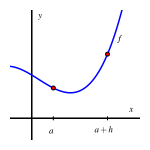
\includegraphics[width=0.5\linewidth]{images/1_3_PA1}
\caption{Plot of \(y = f(x)\) for Preview \hyperref[PA-1-3]{Activity~\ref{PA-1-3}}.\label{F-1-3-PA1}}
\end{figure}
\leavevmode%
\begin{enumerate}[label=\alph*]
\item\hypertarget{li-116}{}Locate and label the points \((a,f(a))\) and \((a+h, f(a+h))\) on the graph.%
\item\hypertarget{li-117}{}Construct a right triangle whose hypotenuse is the line segment from \((a,f(a))\) to \((a+h,f(a+h))\).  What are the lengths of the respective legs of this triangle?%
\item\hypertarget{li-118}{}What is the slope of the line that connects the points \((a,f(a))\) and \((a+h, f(a+h))\)?%
\item\hypertarget{li-119}{}Write a meaningful sentence that explains how the average rate of change of the function on a given interval and the slope of a related line are connected.%
\end{enumerate}
\typeout{************************************************}
\typeout{Subsection 1.3.2 The Derivative of a Function at a Point}
\typeout{************************************************}
\subsection[{The Derivative of a Function at a Point}]{The Derivative of a Function at a Point}\label{subsection-10}

Just as we defined instantaneous velocity in terms of average velocity, we now define the instantaneous rate of change of a function at a point in terms of the average rate of change of the function \(f\) over related intervals. In addition, we give a special name to ``the instantaneous rate of change of \(f\) at \(a\),''\index{} calling this quantity ``the \emph{derivative} of \(f\) at \(a\),'' with this value being represented by the shorthand notation \(f'(a)\). Specifically, we make the following definition.
%
\begin{definition}[{}]\label{def-derivative}

Let \(f\) be a function and \(x = a\) a value in the function's domain. We define the derivative of \(f\) with respect to \(x\) evaluated at \(x = a\)\index{}, denoted \(f'(a)\), by the formula
%
\begin{equation*}
f'(a) = \lim_{h \to 0} \frac{f(a+h)-f(a)}{h},
\end{equation*}\par

provided this limit exists.
%
\end{definition}
\par

Aloud, we read the symbol \(f'(a)\) as either ``\(f\)-prime at \(a\)'' or ``the derivative of \(f\) evaluated at \(x = a\).'' Much of the next several chapters will be devoted to understanding, computing, applying, and interpreting derivatives. For now, we make the following important notes.
%
\leavevmode%
\begin{itemize}[label=\textbullet]
\item{}The derivative of \(f\) at the value \(x = a\) is defined as the limit of the average rate of change of \(f\) on the interval \([a,a+h]\) as \(h \to 0\).  It is possible for this limit not to exist, so not every function has a derivative at every point.%
\item{}We say that a function that has a derivative at \(x = a\) is \emph{differentiable}\index{} at \(x = a\).%
\item{}The derivative is a generalization of the instantaneous velocity of a position function:  when \(y = s(t)\) is a position function of a moving body, \(s'(a)\) tells us the instantaneous velocity of the body at time \(t=a\).%
\item{}Because the units on \(\frac{f(a+h)-f(a)}{h}\) are ``units of \(f\) per unit of \(x\),'' the derivative has these very same units.  For instance, if \(s\) measures position in feet and \(t\) measures time in seconds, the units on \(s'(a)\) are feet per second.%
\item{}Because the quantity \(\frac{f(a+h)-f(a)}{h}\) represents the slope of the line through \((a,f(a))\) and \((a+h, f(a+h))\), when we compute the derivative we are taking the limit of a collection of slopes of lines, and thus the derivative itself represents the slope of a particularly important line.%
\end{itemize}
\par

While all of the above ideas are important and we will add depth and perspective to them through additional time and study, for now it is most essential to recognize how the derivative of a function at a given value represents the slope of a certain line. Thus, we expand upon the last bullet item above.
%
\par

As we move from an average rate of change to an instantaneous one, we can think of one point as ``sliding towards'' another. In particular, provided the function has a derivative at \((a,f(a))\), the point \((a+h,f(a+h))\) will approach \((a,f(a))\) as \(h \to 0\). Because this process of taking a limit is a dynamic one, it can be helpful to use computing technology to visualize what the limit is accomplishing. While there are many different options\footnote{For a helpful collection of java applets, consider the \href{http://gvsu.edu/s/5r}{work of David Austin} of Grand Valley State University, and \href{http://gvsu.edu/s/5s}{this particularly relevant example}.  For applets that have been built in Geogebra, a nice example is the \href{http://gvsu.edu/s/5p}{work of Marc Renault} of Shippensburg University, with \href{http://gvsu.edu/s/5q}{this example} being especially fitting for our work in this section.  There are scores of other examples posted by other authors on the internet.\label{fn-3}}, one of the best is a java applet in which the user is able to control the point that is moving.  %%%SHOULD I EMBED SOMETHING HERE, OR POST THE LINKS OUTSIDE OF FOOTNOTES?%%% See the examples referenced in the footnote here, or consider building your own, perhaps using the fantastic free program Geogebra\footnote{Available for \href{http://geogebra.org}{free download}.\label{fn-4}}.
%
\par

In \hyperref[F-1-3-SecToTanSeq]{Figure~\ref{F-1-3-SecToTanSeq}}, we provide a sequence of figures with several different lines through the points \((a, f(a))\) and \((a+h,f(a+h))\) that are generated by different values of \(h\). These lines (shown in the first three figures in magenta), are often called \emph{secant lines} \index{} to the curve \(y = f(x)\). A secant line to a curve is simply a line that passes through two points that lie on the curve. For each such line, the slope of the secant line is \(m = \frac{f(a+h) - f(a)}{h}\), where the value of \(h\) depends on the location of the point we choose. We can see in the diagram how, as \(h \to 0\), the secant lines start to approach a single line that passes through the point \((a,f(a))\). In the situation where the limit of the slopes of the secant lines exists, we say that the resulting value is the slope of the \emph{tangent line} to the curve. This tangent line\index{} (shown in the right-most figure in green) to the graph of \(y = f(x)\) at the point \((a,f(a))\) is the line through \((a,f(a))\) whose slope is \(m = f'(a)\).
%
\leavevmode%
\begin{figure}
\centering
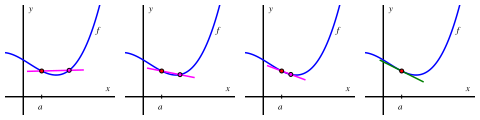
\includegraphics[width=1\linewidth]{images/1_3_SecToTanSeq}
\caption{A sequence of secant lines approaching the tangent line to \(f\) at \((a,f(a))\).\label{F-1-3-SecToTanSeq}}
\end{figure}
\par

As we will see in subsequent study, the existence of the tangent line at \(x = a\) is connected to whether or not the function \(f\) looks like a straight line when viewed up close at \((a,f(a))\), which can also be seen in \hyperref[F-1-3-SecToTan]{Figure~\ref{F-1-3-SecToTan}}, where we combine the four graphs in \hyperref[F-1-3-SecToTanSeq]{Figure~\ref{F-1-3-SecToTanSeq}} into the single one on the left, and then we zoom in on the box centered at \((a,f(a))\), with that view expanded on the right (with two of the secant lines omitted). Note how the tangent line sits relative to the curve \(y = f(x)\) at \((a,f(a))\) and how closely it resembles the curve near \(x = a\).
%
\leavevmode%
\begin{figure}
\centering
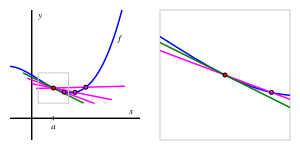
\includegraphics[width=0.75\linewidth]{images/1_3_SecToTan}
\caption{A sequence of secant lines approaching the tangent line to \(f\) at \((a,f(a))\).  At right, we zoom in on the point \((a,f(a))\).  The slope of the tangent line (in green) to \(f\) at \((a,f(a))\) is given by \(f'(a)\).\label{F-1-3-SecToTan}}
\end{figure}
\begin{note}[]\label{note-1}
 \(f'(a)\), the instantaneous rate of change of \(f\) with respect to \(x\) at \(x = a\), also measures the slope of the tangent line to the curve \(y = f(x)\) at \((a,f(a))\). %
\end{note}
\par
The following example demonstrates several key ideas involving the derivative of a function.%
\begin{example}[ Using the limit definition of the derivative
  ]\label{example-3}

For the function given by \(f(x) = x - x^2\), use the limit definition of the derivative to compute \(f'(2)\). In addition, discuss the meaning of this value and draw a labeled graph that supports your explanation.
%
\par\medskip\noindent%
\textbf{Solution.}\quad 
    From the limit definition, we know that
    %
\begin{equation*}
    f'(2) = \lim_{h \to 0} \frac{f(2+h)-f(2)}{h}.
    \end{equation*}\par

    Now we use the rule for \(f\), and observe that \(f(2) = 2 - 2^2 = -2\) and \(f(2+h) = (2+h) - (2+h)^2.\) Substituting these values into the limit definition, we have that
    %
\begin{equation*}
    f'(2) = \lim_{h \to 0} \frac{(2+h) - (2+h)^2 -  (-2)}{h}.
    \end{equation*}\par

    With \(h\) in the denominator and our desire to let \(h \to 0\), we have to wait to take the limit (that is, we wait to actually let \(h\) approach 0). Thus, we do additional algebra. Expanding and distributing in the numerator,
    %
\begin{equation*}
    f'(2) = \lim_{h \to 0} \frac{2+h - 4 - 4h - h^2 + 2}{h}.
    \end{equation*}\par

    Combining like terms, we have
    %
\begin{equation*}
    f'(2) = \lim_{h \to 0} \frac{ -3h - h^2}{h}.
    \end{equation*}\par

    Next, we observe that there is a common factor of \(h\) in both the numerator and denominator, which allows us to simplify and find that
    %
\begin{equation*}
    f'(2) = \lim_{h \to 0} (-3-h).
    \end{equation*}\par

    Finally, we are able to take the limit as \(h \to 0\), and thus conclude that \(f'(2) = -3\).
    %
\par

    Now, we know that \(f'(2)\) represents the slope of the tangent line to the curve \(y = x - x^2\) at the point \((2,-2)\); \(f'(2)\) is also the instantaneous rate of change of \(f\) at the point \((2,-2)\). Graphing both the function and the line through \((2,-2)\) with slope \(m = f'(2) = -3\), we indeed see that by calculating the derivative, we have found the slope of the tangent line at this point, as shown in \hyperref[F-1-3-Ex1]{Figure~\ref{F-1-3-Ex1}}.
    %
\leavevmode%
\begin{figure}
\centering
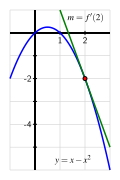
\includegraphics[width=0.5\linewidth]{images/1_3_Ex1}
\caption{The tangent line to \(y = x - x^2\) at the point \((2,-2)\).\label{F-1-3-Ex1}}
\end{figure}
\end{example}
\par

The following activities will help you explore a variety of key ideas related to derivatives.
%
\begin{activity}[The Derivative of a Familiar Function]\label{act-1-3-1}

          Consider the function \(f\) whose formula is \(\displaystyle f(x) = 3 - 2x\).
          %
\leavevmode%
\begin{enumerate}[label=\alph*]
\item\hypertarget{li-125}{}What familiar type of function is \(f\)?  What can you say about the slope of \(f\) at every value of \(x\)?%
\item\hypertarget{li-126}{}Compute the average rate of change of \(f\) on the intervals \([1,4]\), \([3,7]\), and \([5,5+h]\); simplify each result as much as possible.  What do you notice about these quantities?%
\item\hypertarget{li-127}{}Use the limit definition of the derivative to compute the exact instantaneous rate of change of \(f\) with respect to \(x\) at the value \(a = 1\).  That is, compute \(f'(1)\) using the limit definition.  Show your work.  Is your result surprising?%
\item\hypertarget{li-128}{}Without doing any additional computations, what are the values of \(f'(2)\), \(f'(\pi)\), and \(f'(-\sqrt{2})\)?  Why?%
\end{enumerate}
\leavevmode%
\begin{enumerate}[label=\alph*]
\item\hypertarget{li-129}{}If \(f(x) = 3x^2 + 2x - 4\), we say ``\(f\) is quadratic.''  If \(f(x) = 5 e^{2x-1}\), we say ``\(f\) is exponential.''  What do we say about \(f(x) = 3-2x\)?%
\item\hypertarget{li-130}{}Remember that to compute the average rate of change of \(f\) on \([a,b]\), we calculate \(\frac{f(b)-f(a)}{b-a}\).%
\item\hypertarget{li-131}{}Observe that \(f(1+h) = 3 - 2(1+h) = 3 - 2 - 2h = 1 - 2h\).%
\item\hypertarget{li-132}{}Think about the how the graph of \(f\) appears.  What is the same at every point?%
\end{enumerate}
\leavevmode%
\begin{enumerate}[label=\alph*]
\item\hypertarget{li-133}{}\(f\) is linear.%
\item\hypertarget{li-134}{}\(f'(1)=-2\)%
\item\hypertarget{li-135}{}The average rate of change on \([1,4]\), \([3,7]\),  and \([5,5+h]\) is \(-2\). %
\item\hypertarget{li-136}{}\(f'(2)=-2\), \(f'(\pi)=-2\), and \(f'(-\sqrt{2})=-2\), since the slope of a linear function is the same at every point.%
\end{enumerate}
\par\medskip\noindent%
\textbf{Solution.}\quad \leavevmode%
\begin{enumerate}[label=\alph*]
\item\hypertarget{li-137}{}Because \(f(x) = 3 - 2x\) is of the form \(f(x) = mx + b\), we call \(f\) a \emph{linear} function.%
\item\hypertarget{li-138}{}The average rate of change on \([1,4]\) is \(\frac{f(4)-f(1)}{4-1} = \frac{-5 - 1}{3} = -2\).  Similar calculations show the average rate of change on \([3,7]\) is also \(-2\).  On \([5,5+h]\), observe that 
            
            \begin{align*}
\frac{f(5+h)-f(5)}{h} \amp = \frac{3-2(5+h) - (3-10)}{h}\\
                      \amp = \frac{3 - 10 - 2h + 7}{h}\\
                      \amp = \frac{-2h}{h} \\
                      \amp = -2.
\end{align*}%
\item\hypertarget{li-139}{}Using the limit definition of the derivative, we find that
            
            \begin{align*}
f'(1) = \amp  \lim_{h \to 0} \frac{f(1+h) - f(1)}{h}\\
         = \amp  \lim_{h \to 0} \frac{(3 - 2(1+h)) - (3-2)}{h}\\
         = \amp  \lim_{h \to 0} \frac{3 - 2 - 2h - 1}{h}\\
         = \amp  \lim_{h \to 0} \frac{-2h}{h}\\
         = \amp  \lim_{h \to 0} -2\\
         = \amp  -2.
\end{align*}%
\end{enumerate}
\end{activity}
\begin{activity}[A Water Balloon]\label{act-1-3-2}

        A water balloon is tossed vertically in the air from a window. The balloon's height in feet at time \(t\) in seconds after being launched is given by \(s(t) = -16t^2 + 16t + 32\). Use this function to respond to each of the following questions.
        %
\leavevmode%
\begin{enumerate}[label=\alph*]
\item\hypertarget{li-140}{}Sketch an accurate, labeled graph of \(s\) on the axes provided in \hyperref[F-1-3-Act2]{Figure~\ref{F-1-3-Act2}}.  You should be able to do this without using computing technology.
            \leavevmode%
\begin{figure}
\centering
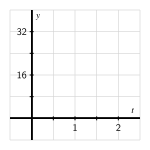
\includegraphics[width=0.5\linewidth]{images/1_3_Act2}
\caption{Axes for plotting \(y = s(t)\) in \hyperref[act-1-3-2]{Activity~\ref{act-1-3-2}}.\label{F-1-3-Act2}}
\end{figure}
%
\item\hypertarget{li-141}{}Compute the average rate of change of \(s\) on the time interval \([1,2]\).  Include units on your answer and write one sentence to explain the meaning of the value you found.%
\item\hypertarget{li-142}{}Use the limit definition to compute the instantaneous rate of change of \(s\) with respect to time, \(t\), at the instant \(a = 1\).  Show your work using proper notation, include units on your answer, and write one sentence to explain the meaning of the value you found.%
\item\hypertarget{li-143}{}On your graph in (a), sketch two lines:  one whose slope represents the average rate of change of \(s\) on \([1,2]\), the other whose slope represents the instantaneous rate of change of \(s\) at the instant \(a=1\).  Label each line clearly.%
\item\hypertarget{li-144}{}For what values of \(a\) do you expect \(s'(a)\) to be positive?  Why?  Answer the same questions when ``positive'' is replaced by ``negative'' and  ``zero.''%
\end{enumerate}
\leavevmode%
\begin{enumerate}[label=\alph*]
\item\hypertarget{li-145}{}Observe that \((t^2 - t - 2) = (t-2)(t+1)\) and that \(s(t)\) has its vertex at \(t = \frac{1}{2}\).%
\item\hypertarget{li-146}{}Recall the formula for average rate of change.%
\item\hypertarget{li-147}{}Note that \(s(1+h) = -16(1+h)^2 + 16(1+h) + 32\).%
\item\hypertarget{li-148}{}Think about a secant line and a tangent line.%
\item\hypertarget{li-149}{}A line with positive slope is one that is rising; a line with negative slope is one that is falling.%
\end{enumerate}
 This %
\par\medskip\noindent%
\textbf{Solution.}\quad \leavevmode%
\begin{enumerate}[label=\alph*]
\item\hypertarget{li-150}{}Since \(s(t) = -16t^2 + 16t + 32 = -16(t^2 - t - 2) = -16(t-2)(t+1)\), \(s\) has \(t\)-intercepts at \((2,0)\) and \((-1,0)\); the \(s\)-intercept is clearly \((0,32)\); and the vertex is \((\frac{1}{2},36)\).  See more in \hyperref[F-1-3-Act2-soln]{Figure~\ref{F-1-3-Act2-soln}}.%
\item\hypertarget{li-151}{}Observe that \(\frac{s(2)-s(1)}{2-1} = \frac{0 - 32}{1} = -32\) feet per second.  This value represents the average rate at which the ball is falling over the time interval from \(t = 1\) to \(t = 2\).%
\item\hypertarget{li-152}{}We compute \(s'(1)\) as follows:
            
            \begin{align*}
s'(1) = \amp  \lim_{h \to 0} \frac{s(1+h)-s(1)}{h}\\
   = \amp  \lim_{h \to 0} \frac{(-16(1+h)^2 + 16(1+h) + 32) - (-16(1)^2 + 16(1) + 32)}{h}\\
   = \amp  \lim_{h \to 0} \frac{-16 - 32h - 16h^2 + 16 + 16h + 32 - 32}{h}\\
   = \amp  \lim_{h \to 0} \frac{-16h - 16h^2}{h}\\
   = \amp  \lim_{h \to 0} (-16-16h)\\
   = \amp  -16.
\end{align*}%
\item\hypertarget{li-153}{}We plot and label the secant line through \((1,s(1))\) and \((2,s(2))\), as well as the tangent line through \((1,s(1))\) with slope \(s'(1)\).
              \leavevmode%
\begin{figure}
\centering
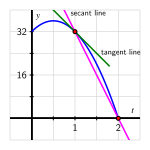
\includegraphics[width=0.5\linewidth]{images/1_3_Act2Soln}
\caption{Graph of \(y = s(t)\) in \hyperref[act-1-3-2]{Activity~\ref{act-1-3-2}}, along with the two lines requested in (d).\label{F-1-3-Act2-soln}}
\end{figure}
%
\item\hypertarget{li-154}{}Observe that whenever the ball is rising, its position function is rising, and thus the slope of its tangent line at any such point will be positive. This means that we should find \(s'(a)\) to be positive whenever \(0 \le a \lt  \frac{1}{2}\), and similarly \(s'(a)\) to be negative whenever \(\frac{1}{2} \lt  a \lt  2\) (which is when the ball is falling).  At the instant \(a = \frac{1}{2}\), the ball is at its vertex and is neither rising nor falling, and at that point, \(s'(\frac{1}{2}) = 0.\)%
\end{enumerate}
\end{activity}
\typeout{************************************************}
\typeout{Subsection 1.3.3 Summary}
\typeout{************************************************}
\subsection[{Summary}]{Summary}\label{subsection-11}
\leavevmode%
\begin{itemize}[label=\textbullet]
\item{}%
\end{itemize}
%
\backmatter
%
%
%% A lineskip in table of contents as transition to appendices, backmatter
\addtocontents{toc}{\vspace{\normalbaselineskip}}
%
%
%% The index is here, setup is all in preamble
\printindex
%
\cleardoublepage
\pagestyle{empty}
\vspace*{\stretch{1}}
\centerline{This book was authored in MathBook XML.%
}
\vspace*{\stretch{2}}
\end{document}